%%% TITLE AND AUTHORS %%%%%%%%%%%%%%%%%%%%%%%%%%%%%%%%%%%%%%%%%%%%%%%%%%%%%%%%%
\title[Tools of the Trade]{
    Tools of the trade for a computational social scientist \\
    \small{}
}
\author[]{Szymon Talaga and Mikołaj Biesaga} % Your name
\institute[ISS UW]{
    The Robert Zajonc Institute for Social Studies \\ University of Warsaw \\
    \medskip
    \textcolor{blue}{\href{mailto:stalaga@uw.edu.pl}{stalaga@uw.edu.pl}} \\
    \textcolor{blue}{\href{mailto:m.biesaga@uw.edu.pl}{m.biesaga@uw.edu.pl}}
}
\date{16 October 2019} % Date, can be changed to a custom date

%%% SLIDES %%%%%%%%%%%%%%%%%%%%%%%%%%%%%%%%%%%%%%%%%%%%%%%%%%%%%%%%%%%%%%%%%%%%
\frame{\titlepage}

\section[R]{R}

\begin{frame}
    \only<1>{
        \centering
    
\includegraphics[scale = .2]{png/r_logo.png}
    }
    \only<2>{
        \frametitle{What is R?}
        \begin{definition}
            \emph{R} is a programming language and free software environment for statistical computing and graphics. The capabilities of R are extended through user-created packages, which allow specialized statistical techniques, graphical devices, import/export capabilities, reporting tools, etc. The core set of packages is installed in every distribution of R, and thousands more are available on Comprehensive R Archive Network (CRAN), Bioconductor, GitHub, and other repositories.
        \end{definition}
    }
    \only<3,5>{
        \frametitle{How to install R on Mac?}
        To install R just follow these eight easy steps:
        \begin{enumerate}
            \item<3,5> Visit \textcolor{blue}{\href{https://www.r-project.org}{www.r-project.org}}
            \item<3,5> Click download R
            \item<3,5> Choose the closest mirror (in geographic sense)
            \item<3,5> Click Download R for (Mac) OS X
            \item<3,5> Choose the latest stable (recommended) version and download it
            \item<3,5> Download also XQuartz
            \item<5> Double click on \mintinline{bash}{R-3.6.1.pkg} and follow the default installation
            \item<5> Double click on \mintinline{bash}{XQuartz_2.7.11.dmg} and follow the default installation
        \end{enumerate}
    }
    \only<4>{
        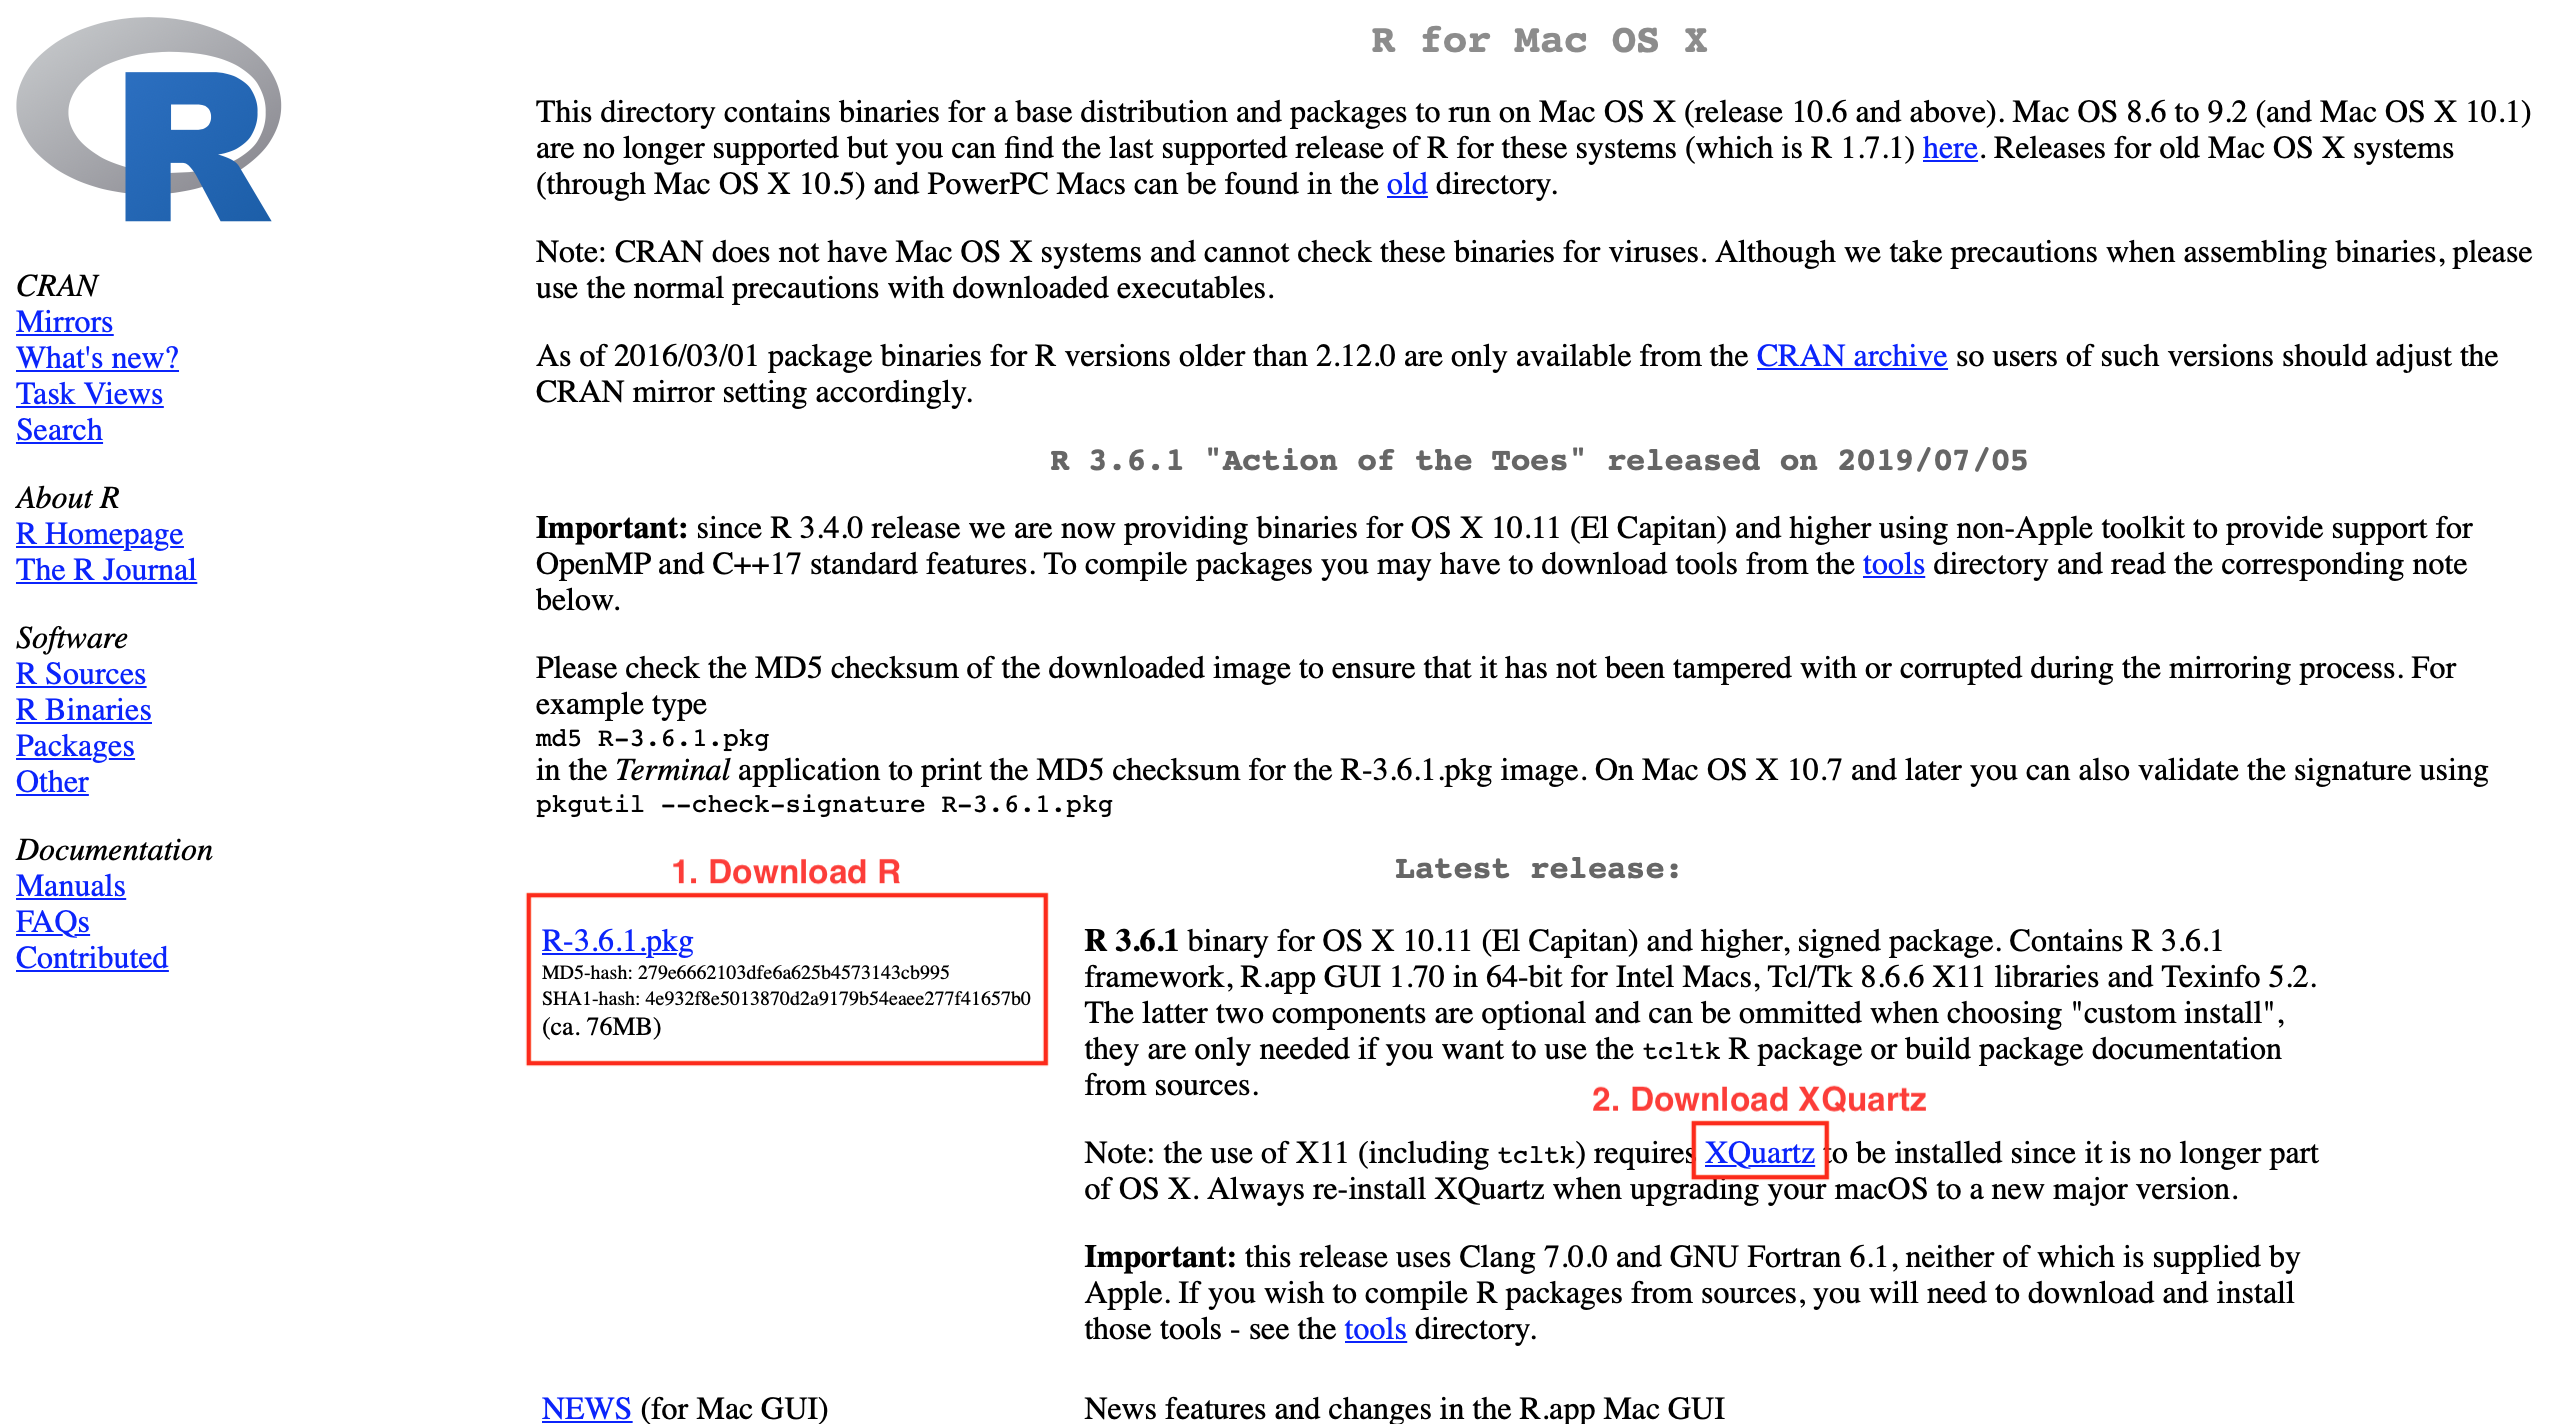
\includegraphics[width = \framewidth]{png/mac_users.png}
    }
    \only<6,8>{
        \frametitle{How to install R on Windows?}
        To install R just follow these six easy steps:
        \begin{enumerate}
            \item<6,8> Visit \textcolor{blue}{\href{https://www.r-project.org}{www.r-project.org}}
            \item<6,8> Click download R
            \item<6,8> Choose the closest mirror (in geographic sense)
            \item<6,8> Click Download R for Windows
            \item<6,8> Choose base and download the latest version
            \item<6,8> Download also RTools (choose the recommended version)
            \item<8> Double click on \mintinline{bash}{R-3.6.1-win.exe} and follow the default installation
            \item<8> Double click on \mintinline{bash}{Rtools35.exe} and follow the default installation
        \end{enumerate}
    }
    \only<7>{
        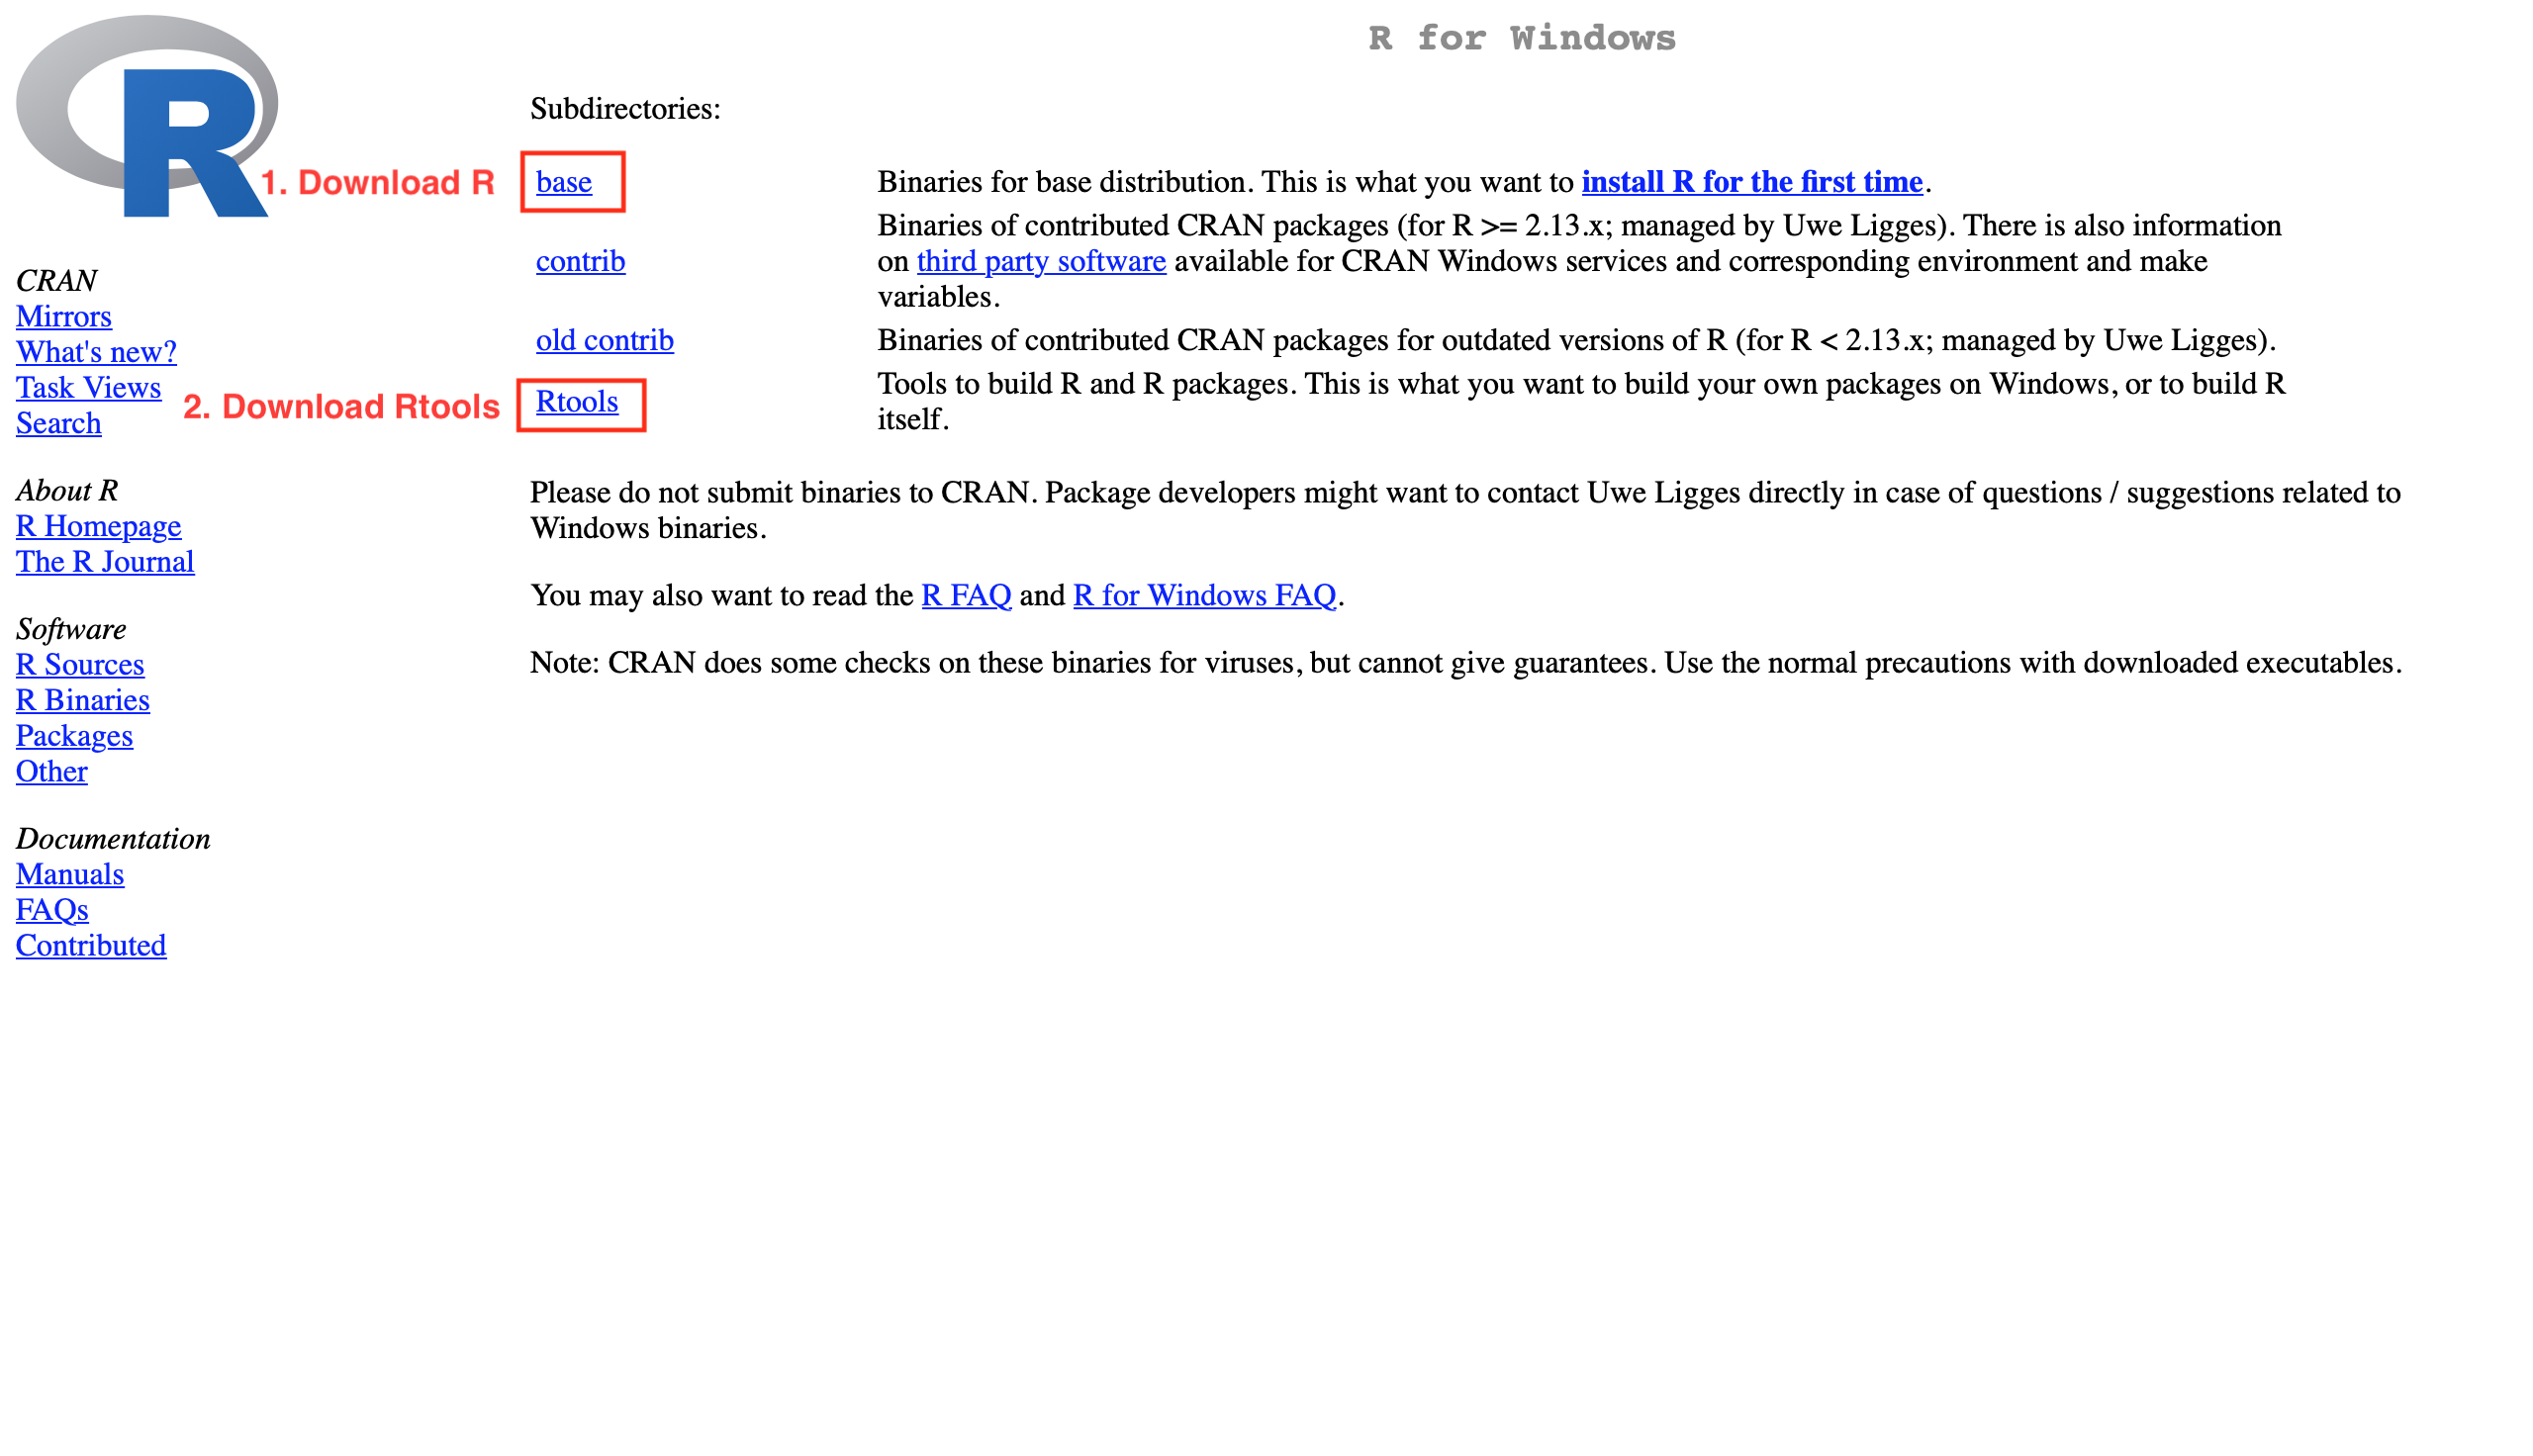
\includegraphics[width = \framewidth]{png/windows_user.png}
    }
    \only<9>{
        \frametitle{Voila!}
        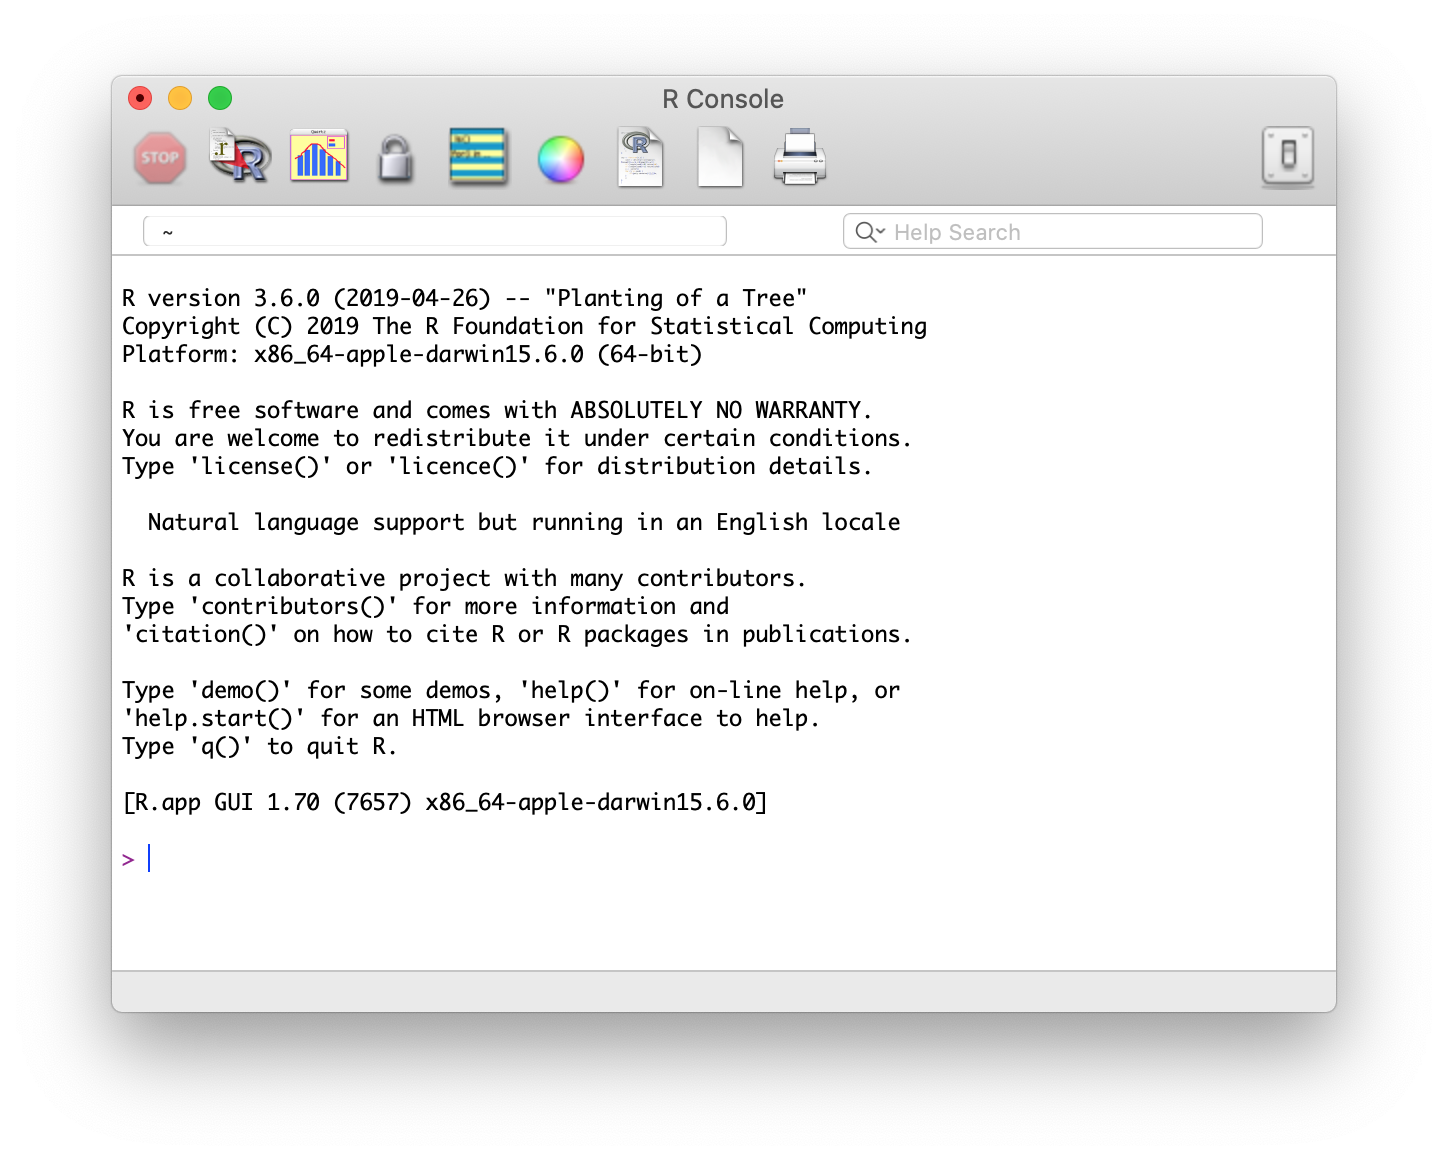
\includegraphics[width = \framewidth]{png/r_desktop.png}
    }
\end{frame}

\subsection[RStudio]{RStudio}

\begin{frame}[fragile]
    \only<1>{
        \centering
        
\includegraphics[width = \framewidth]{png/rstudio_logo.png}
    }
    \only<2>{
        \frametitle{What is RStudio?}
        \emph{RStudio} is an integrated development environment (IDE) for R. In other words, it is a program that allows you to write and execute R scripts in a more than convenient way.
    }
    \only<3,5,7>{
        \frametitle{How to install RStudio?}
        To install RStudio you need to \alert{have R installed} and follow these six easy steps:
        \begin{enumerate}
            \item<3,5,7> Visit \textcolor{blue}{\href{https://rstudio.com/products/rstudio/download/}{www.rstudio.com}}
            \item<3,5,7> Click download
            \item<3,5,7> Choose RStudio Desktop (the free version)
            \item<5,7> Download version appropriate for your operating system (Windows or macOS)
            \item<7> When the \mintinline{bash}{RStudio-1.2.5001} is downloaded double click on it and follow the default installation
        \end{enumerate}
    }
    \only<4>{
        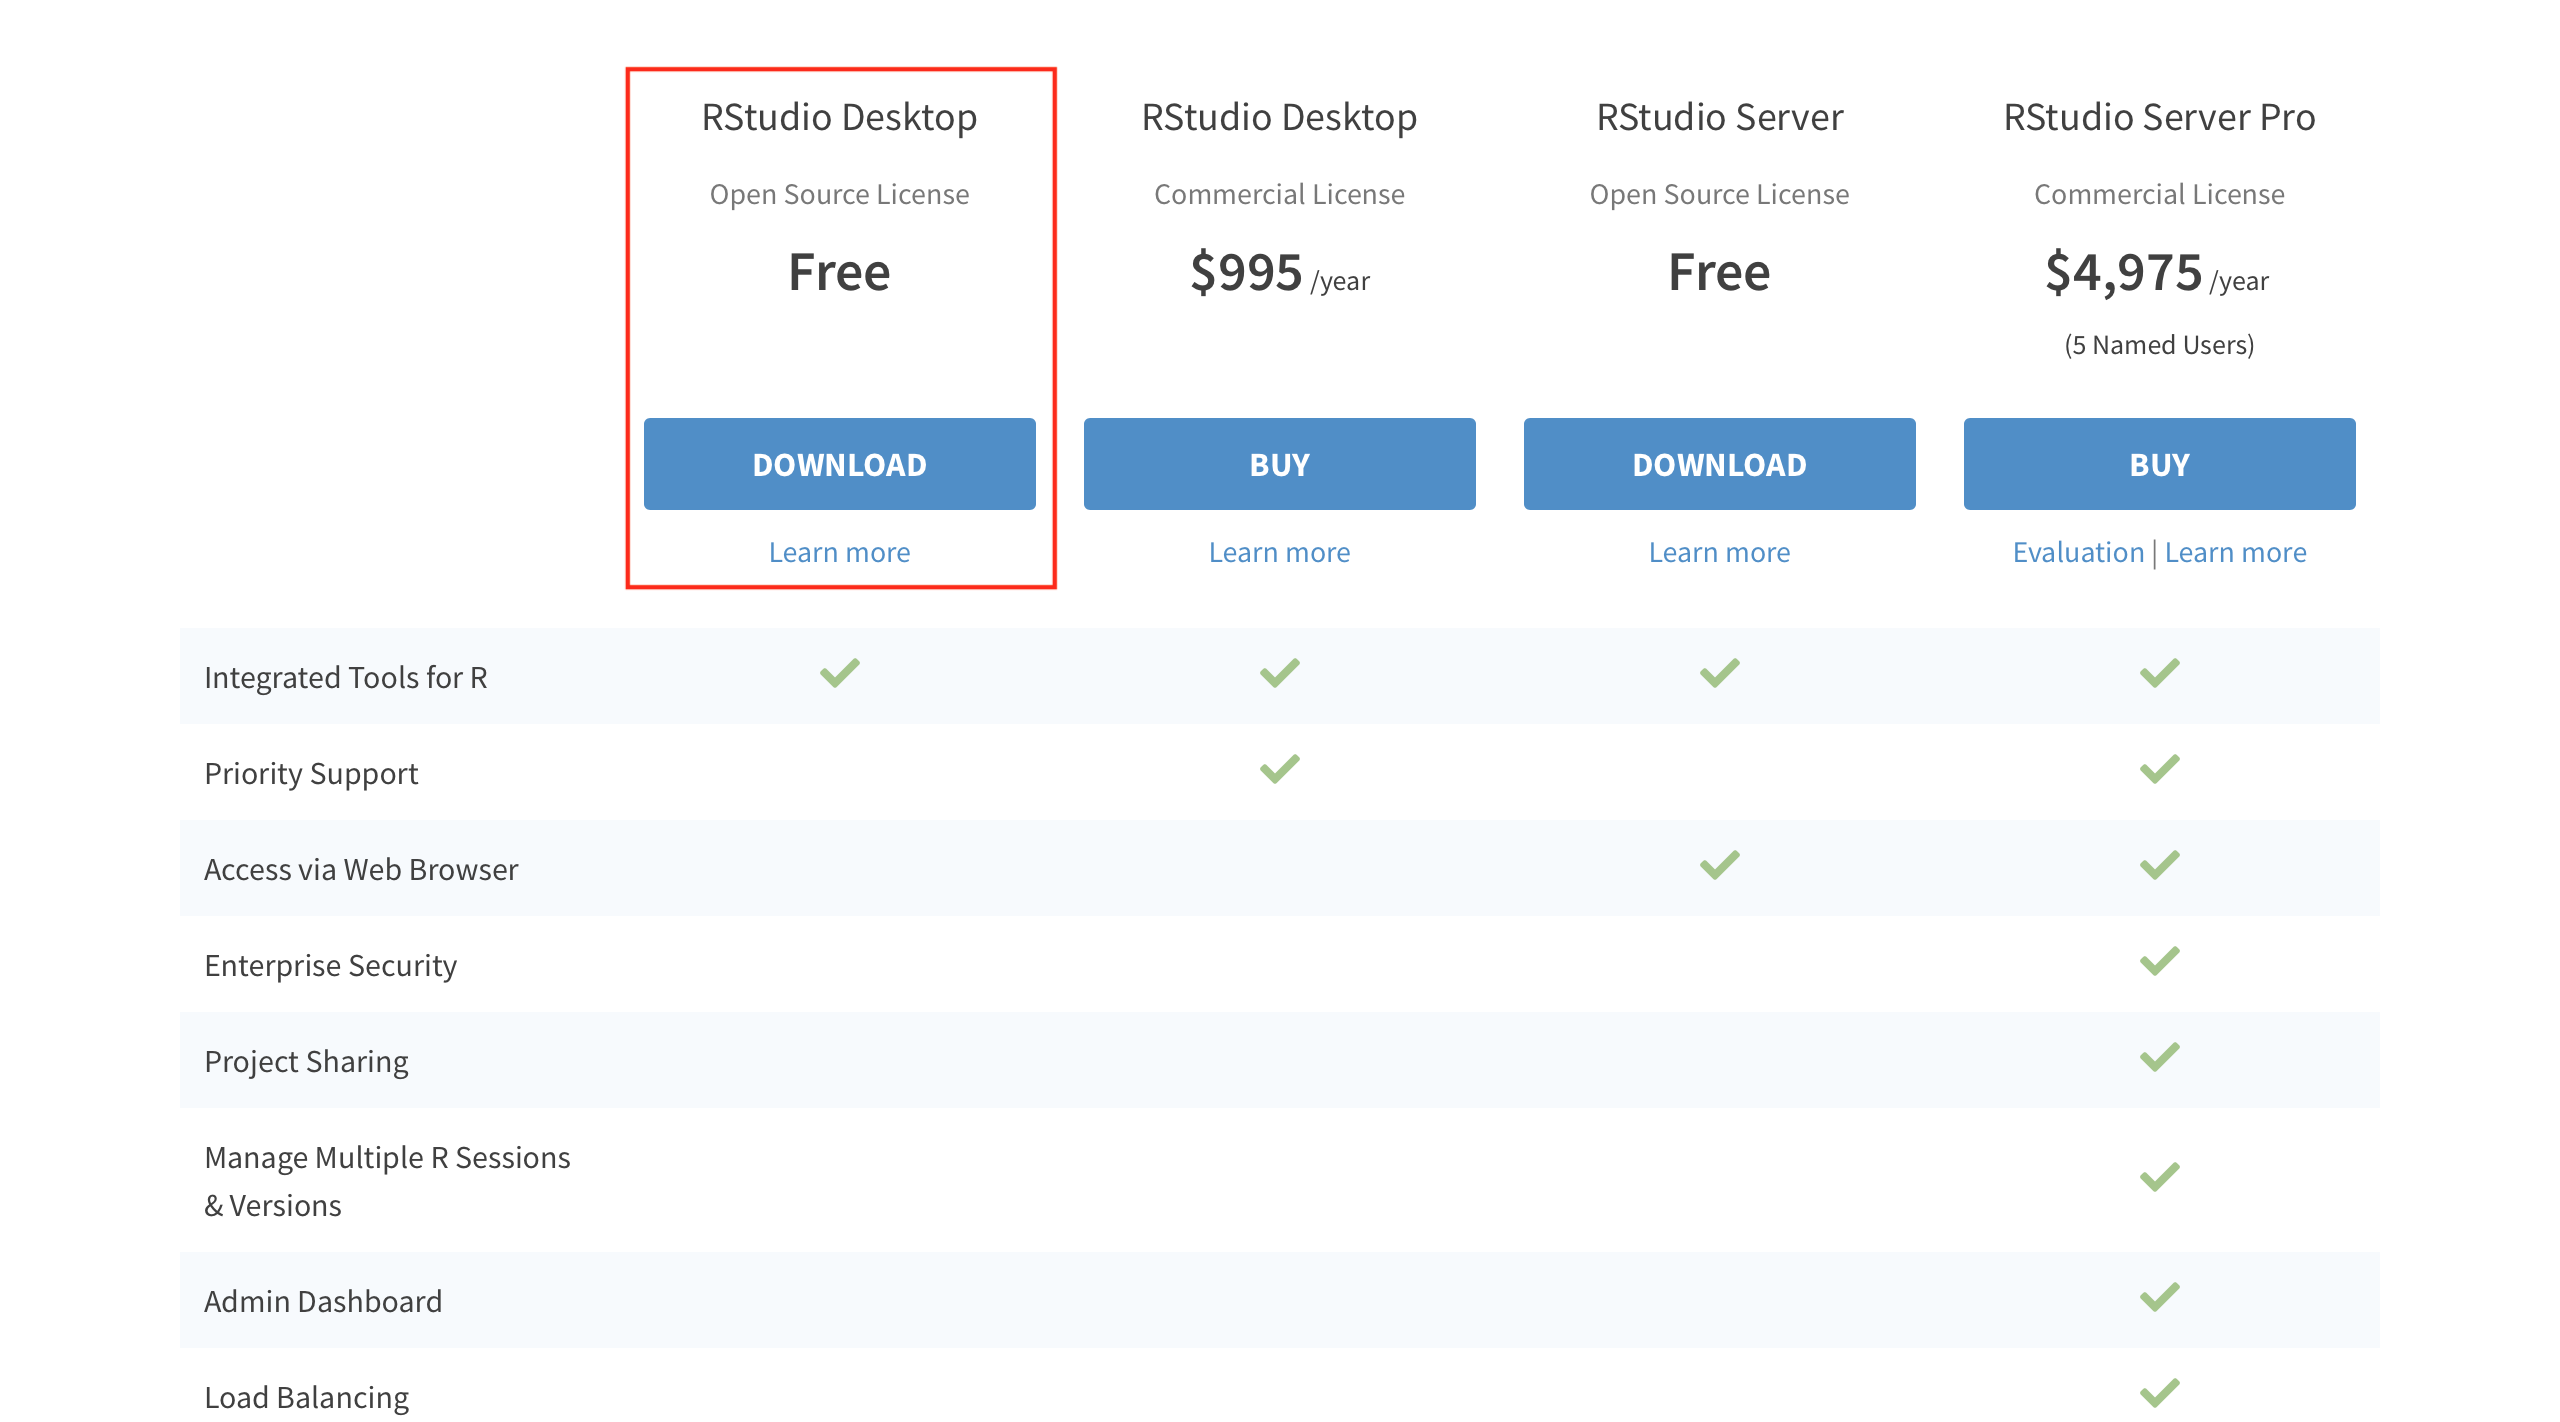
\includegraphics[width = \framewidth]{png/rstudio_download.png}
    }
    \only<6>{
        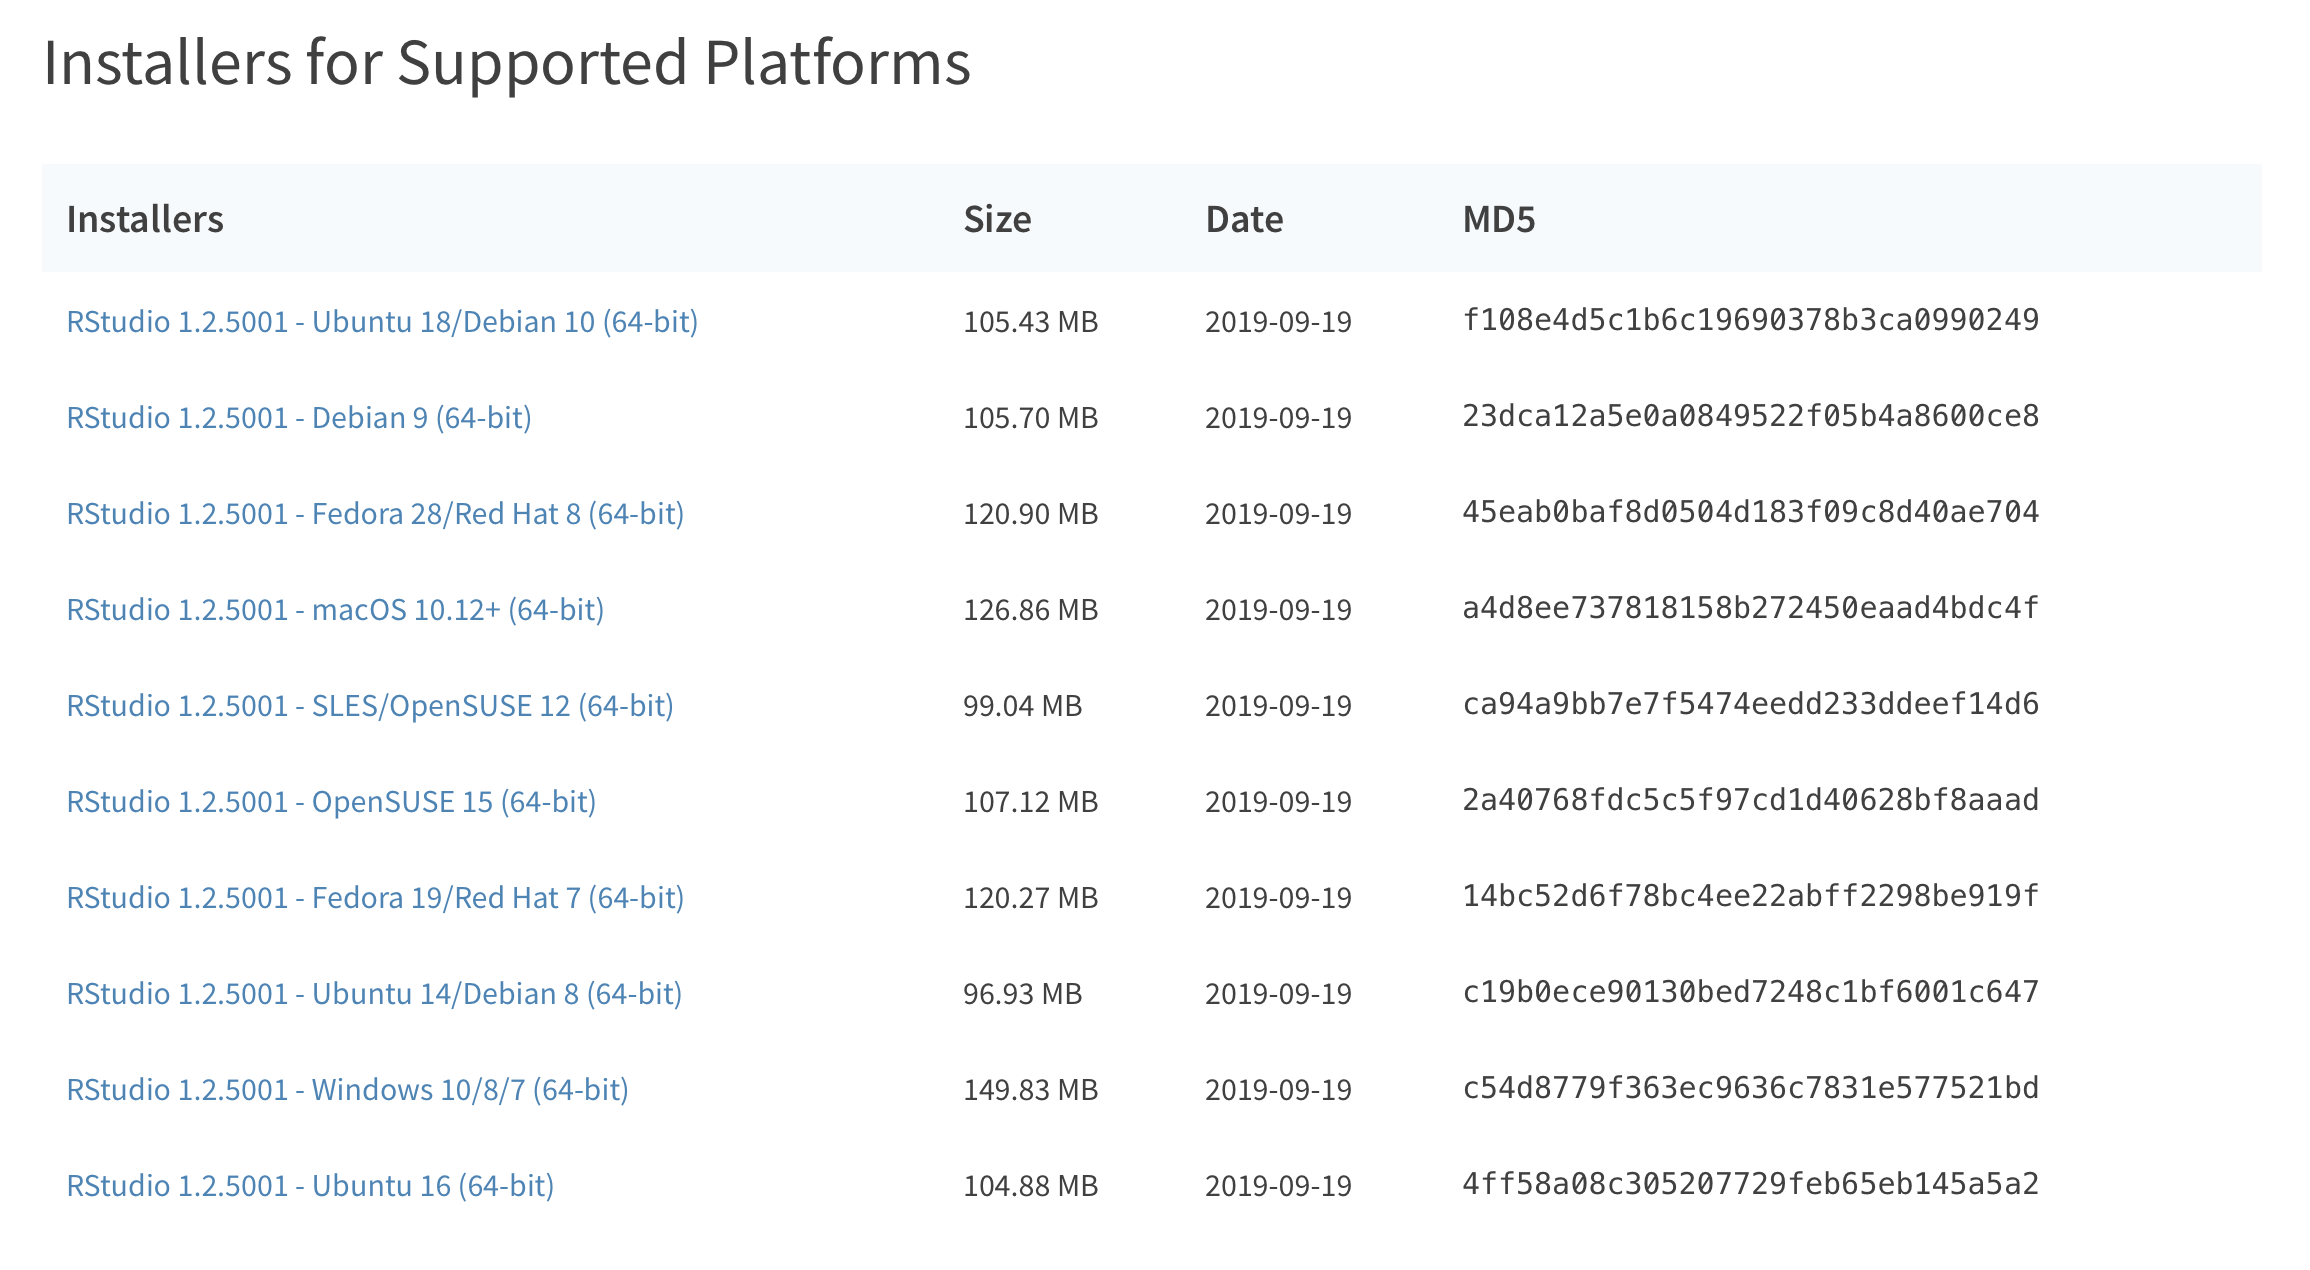
\includegraphics[width = \framewidth]{png/rstudio_download_2.png}
    }
    \only<8>{
        \frametitle{Voila!}
        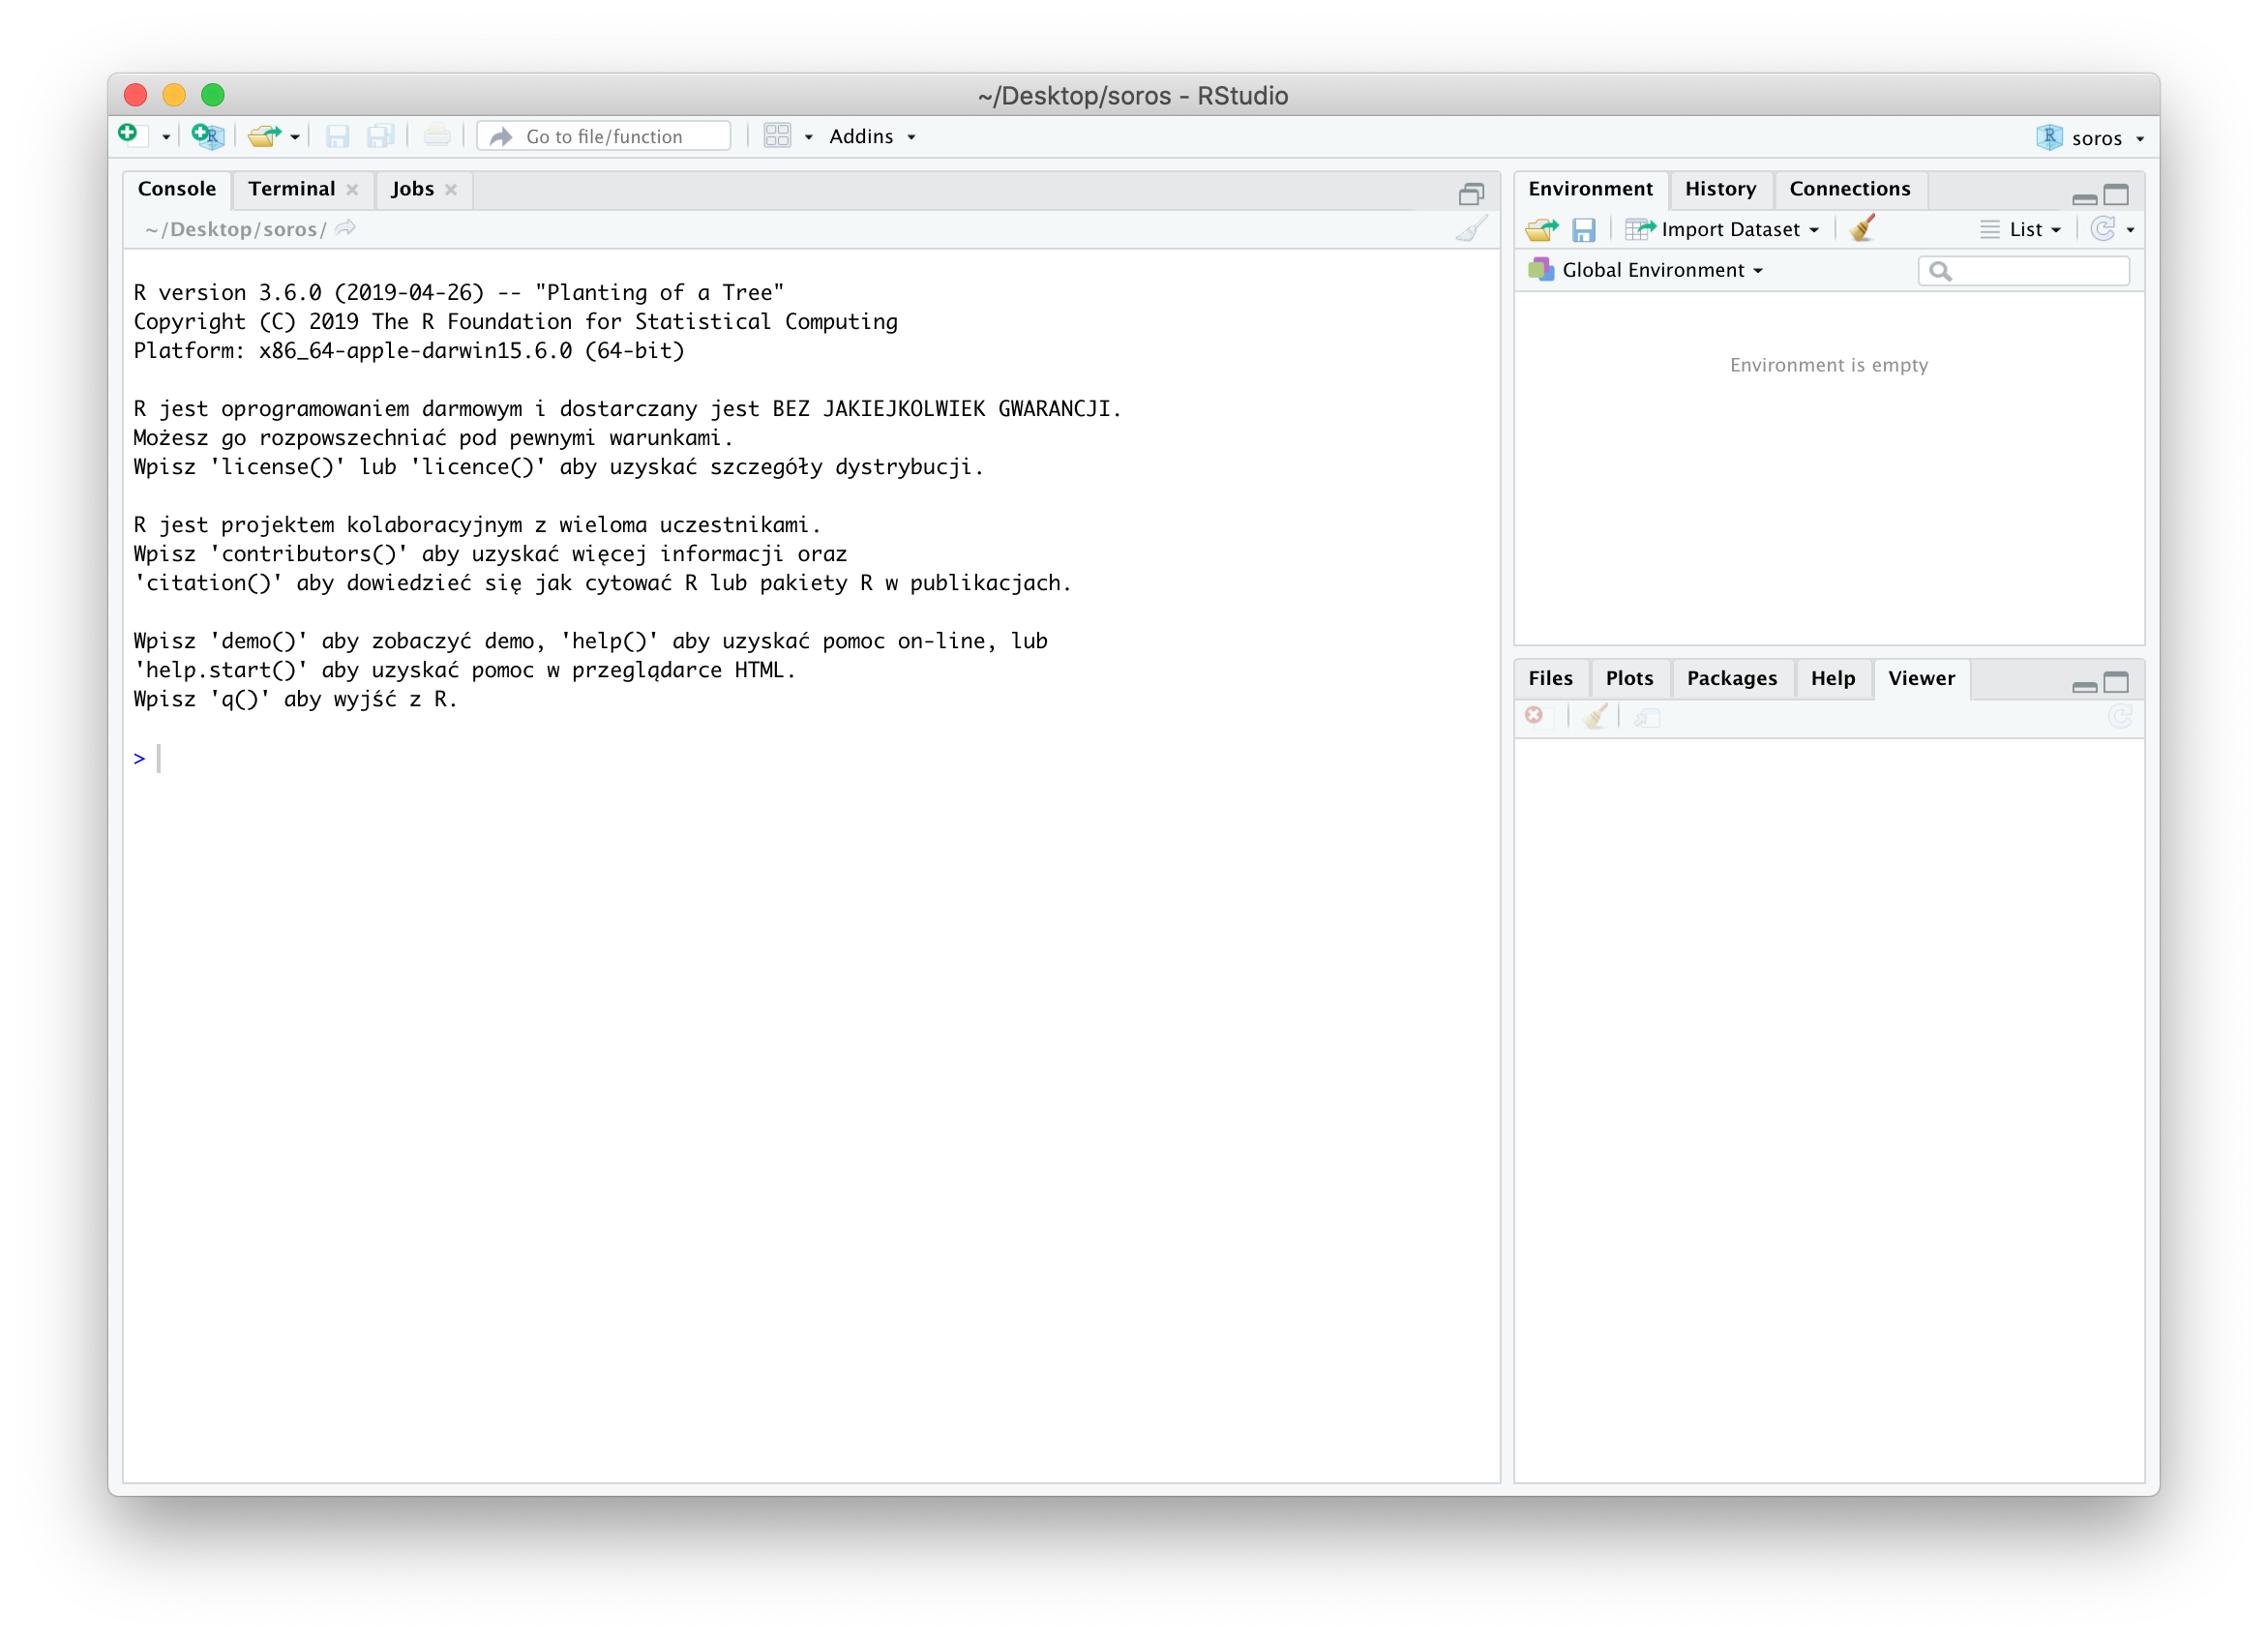
\includegraphics[width = \framewidth]{png/rstudio.png}
    }
\end{frame}

\section[Python]{Python}

\begin{frame}
    \only<+>{
        \centering
        
\includegraphics[width = \framewidth]{png/python_logo.png}
    }
    \only<+>{
        \frametitle{What is Python?}
        \begin{definition}
            \emph{Python} is a programming language and the Python interpreter software that reads the source code and performs its instructions. There are two generations of Python: Python 2.x and Python 3.x. \alert{We will use Python 3.x only.}
        \end{definition}
    }
    \only<+>{
        \frametitle{Python}
        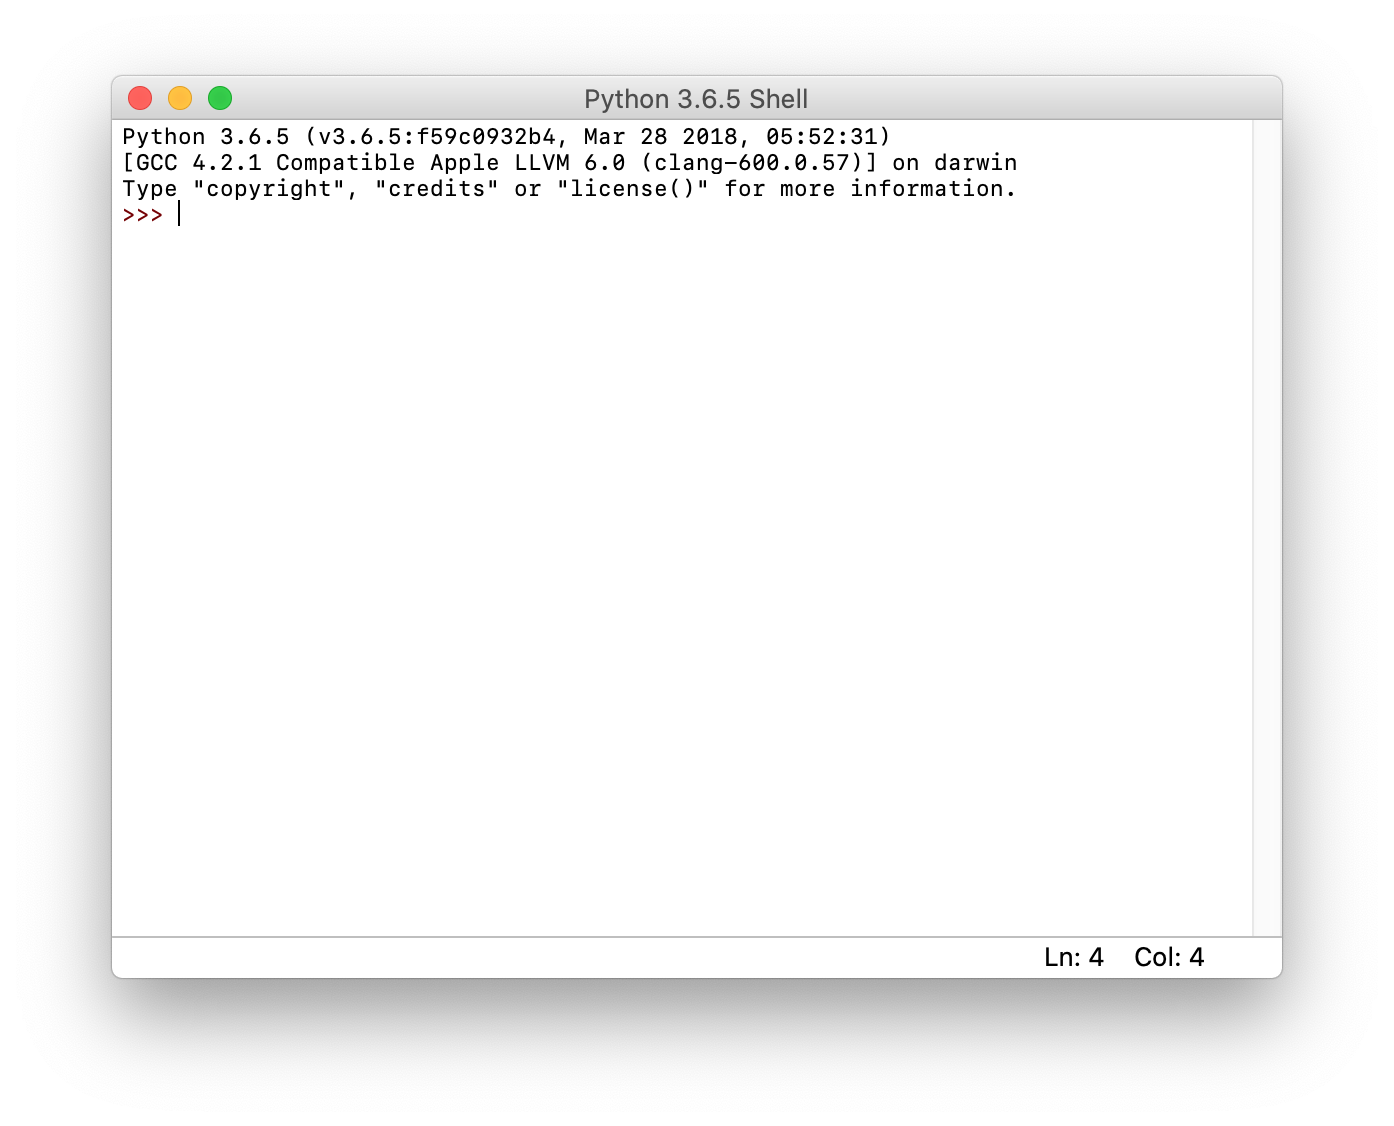
\includegraphics[width = \framewidth]{png/python_idle.png}
    }
\end{frame}
\subsection[Jupyter Notebook]{Jupyter Notebook}
\begin{frame}
    \only<+>{
        \centering
        
\includegraphics[width = .6\framewidth]{png/jupyter.png}
    }
    \only<+>{
        \frametitle{What is Jupyter Notebook?}
        \begin{definition}
            \emph{Jupyter Notebooks} are documents produced by the Jupyter Notebook App which contain both computer code (e.g. python) and rich text elements (paragraph, equations, figures, links, etc.). Notebook documents are both human-readable documents containing the analysis description and the results (figures, tables, etc.) as well as executable documents that can be run to perform data analysis.
        \end{definition}
    }
    \only<+>{
        \frametitle{Jupyter Notebook}
        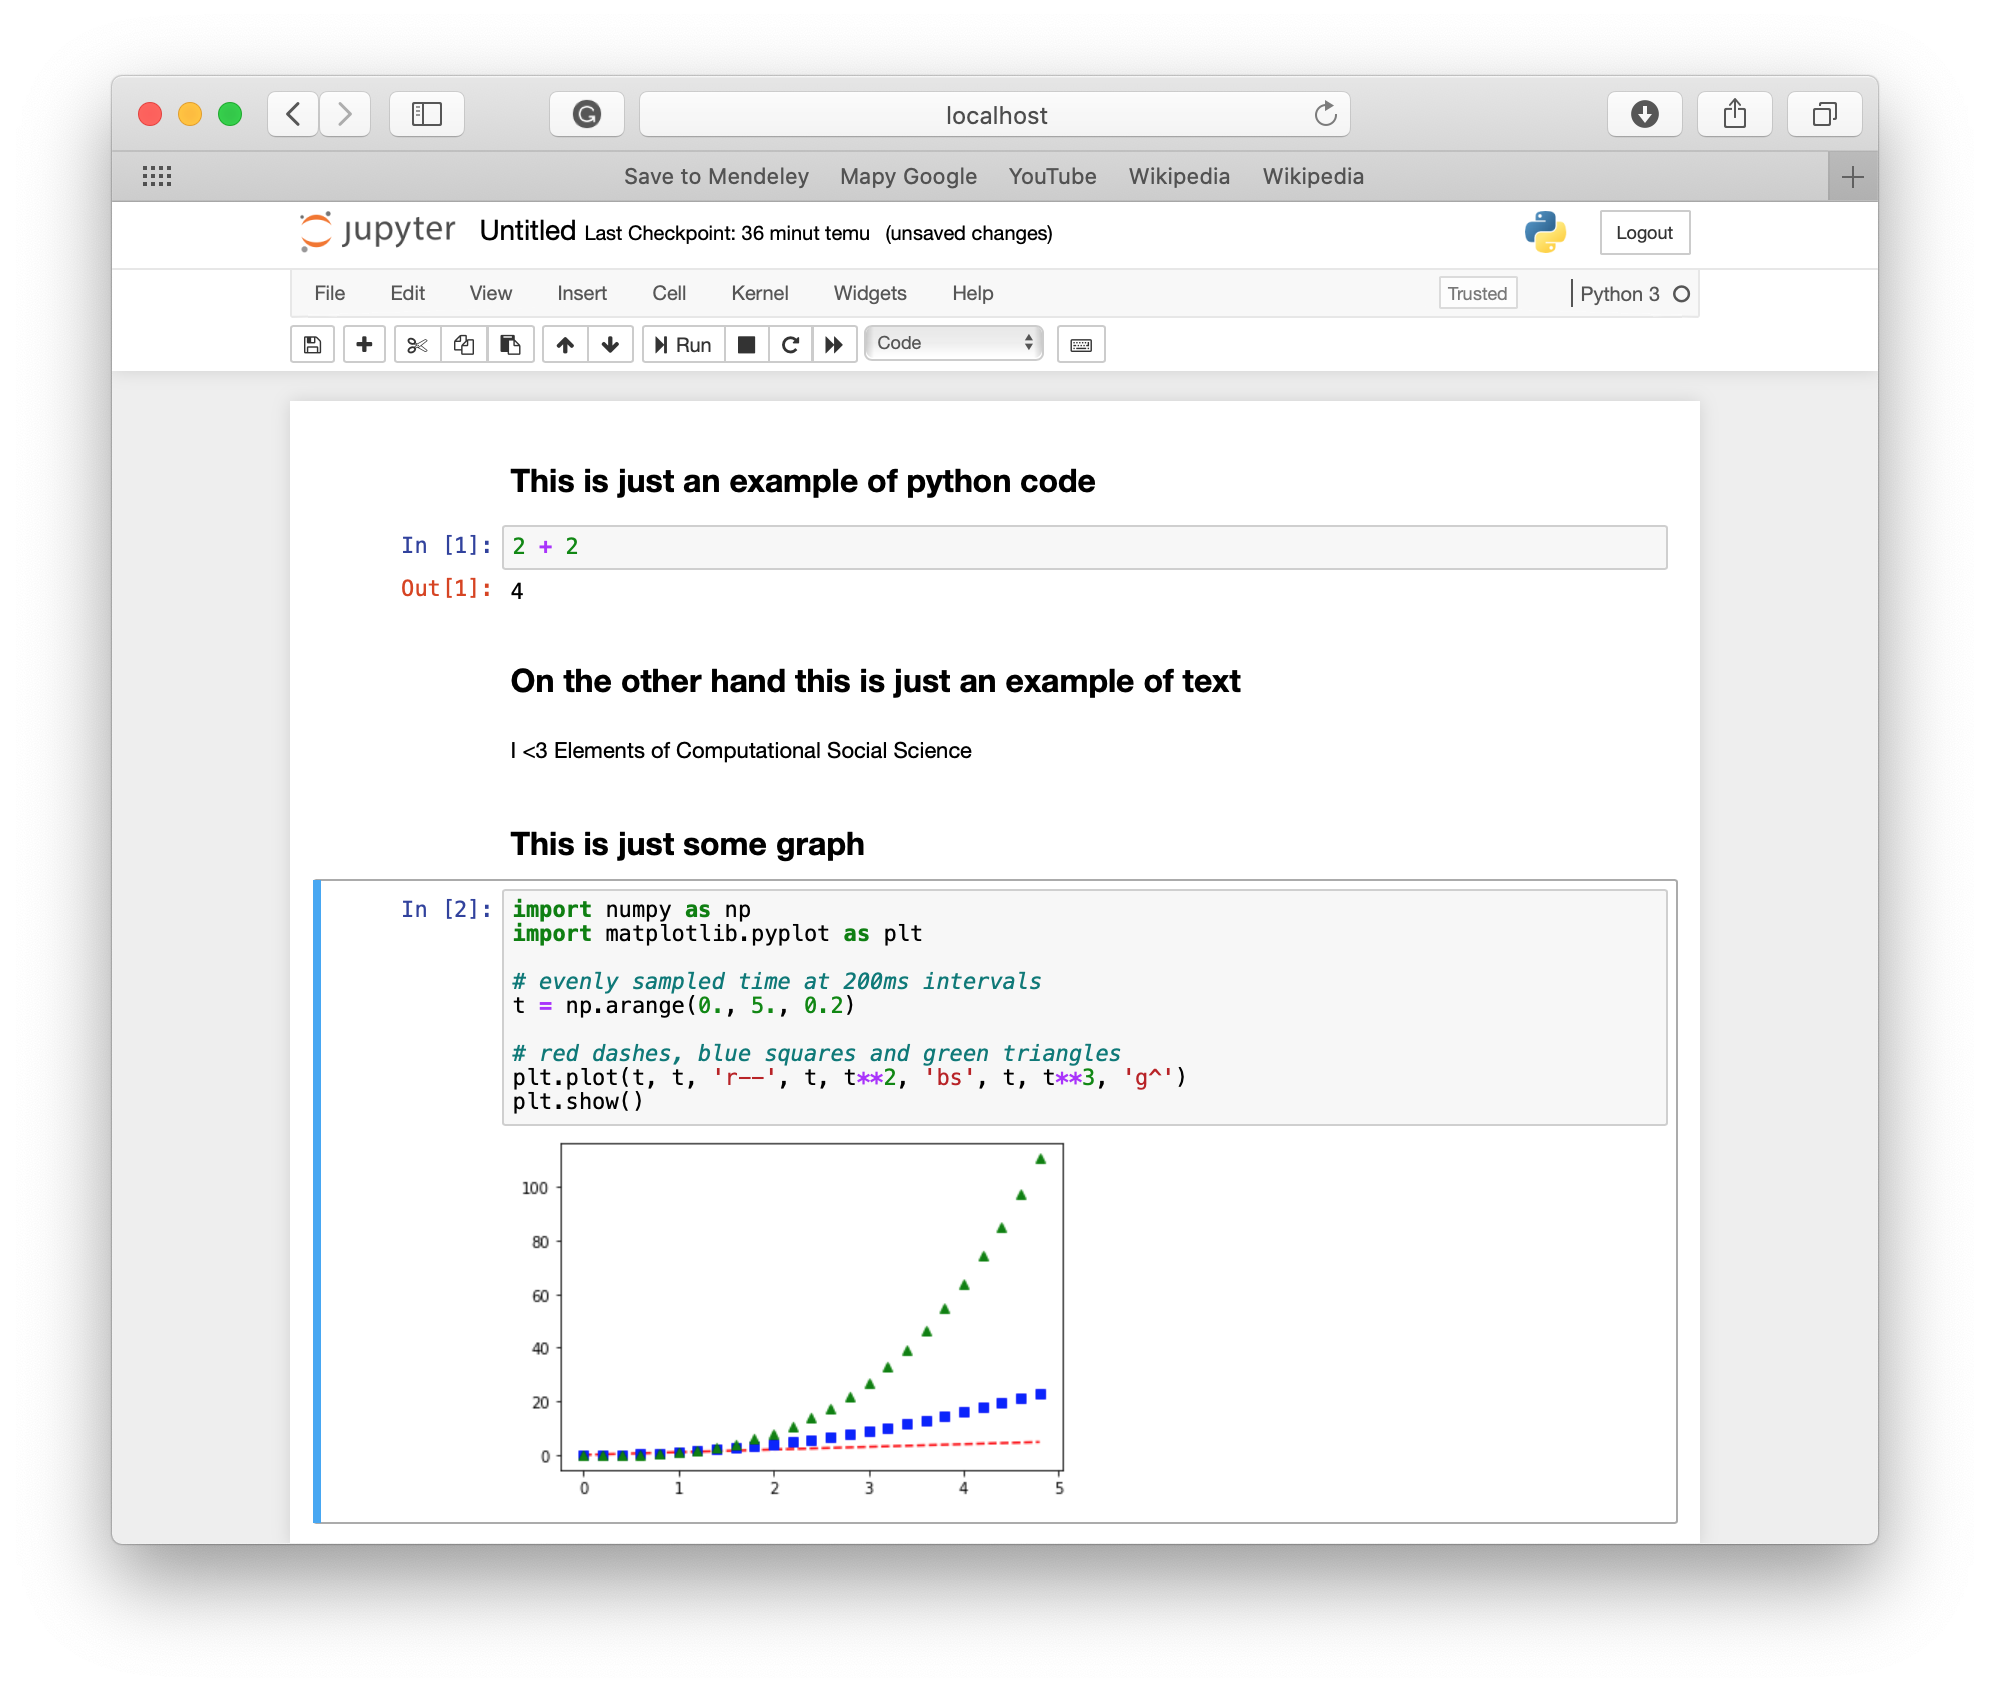
\includegraphics[width = \framewidth]{png/jupyter_notebook.png}
    }
    \only<+>{
        \frametitle{What is Jupyter Notebook App?}
        \begin{definition}
            \emph{The Jupyter Notebook App} is an application that allows editing and running code via a web browser. The app can be run on a local desktop requiring no internet access or can be installed on a remote server and accessed through the internet.
        \end{definition}
    }
\end{frame}

\subsection[Colaboratory]{Colaboratory}
\begin{frame}[fragile]
    \only<+>{
        \begin{center}
            
\includegraphics[scale = .7]{png/colab.png}
        \end{center}
    }
    \only<+>{
        \frametitle{What is Colaboratory?}
        \begin{definition}
            \emph{Colaboratory} is a free Jupyter Notebook environment that requires no setup and runs entirely in the cloud. In other words, it is almost the same as Jupyter Notebook App but it runs in Google Cloud, so if you have a google account you have access to Colaboratory.
        \end{definition}
    }
    \only<+>{
        \frametitle{Colaboratory}
        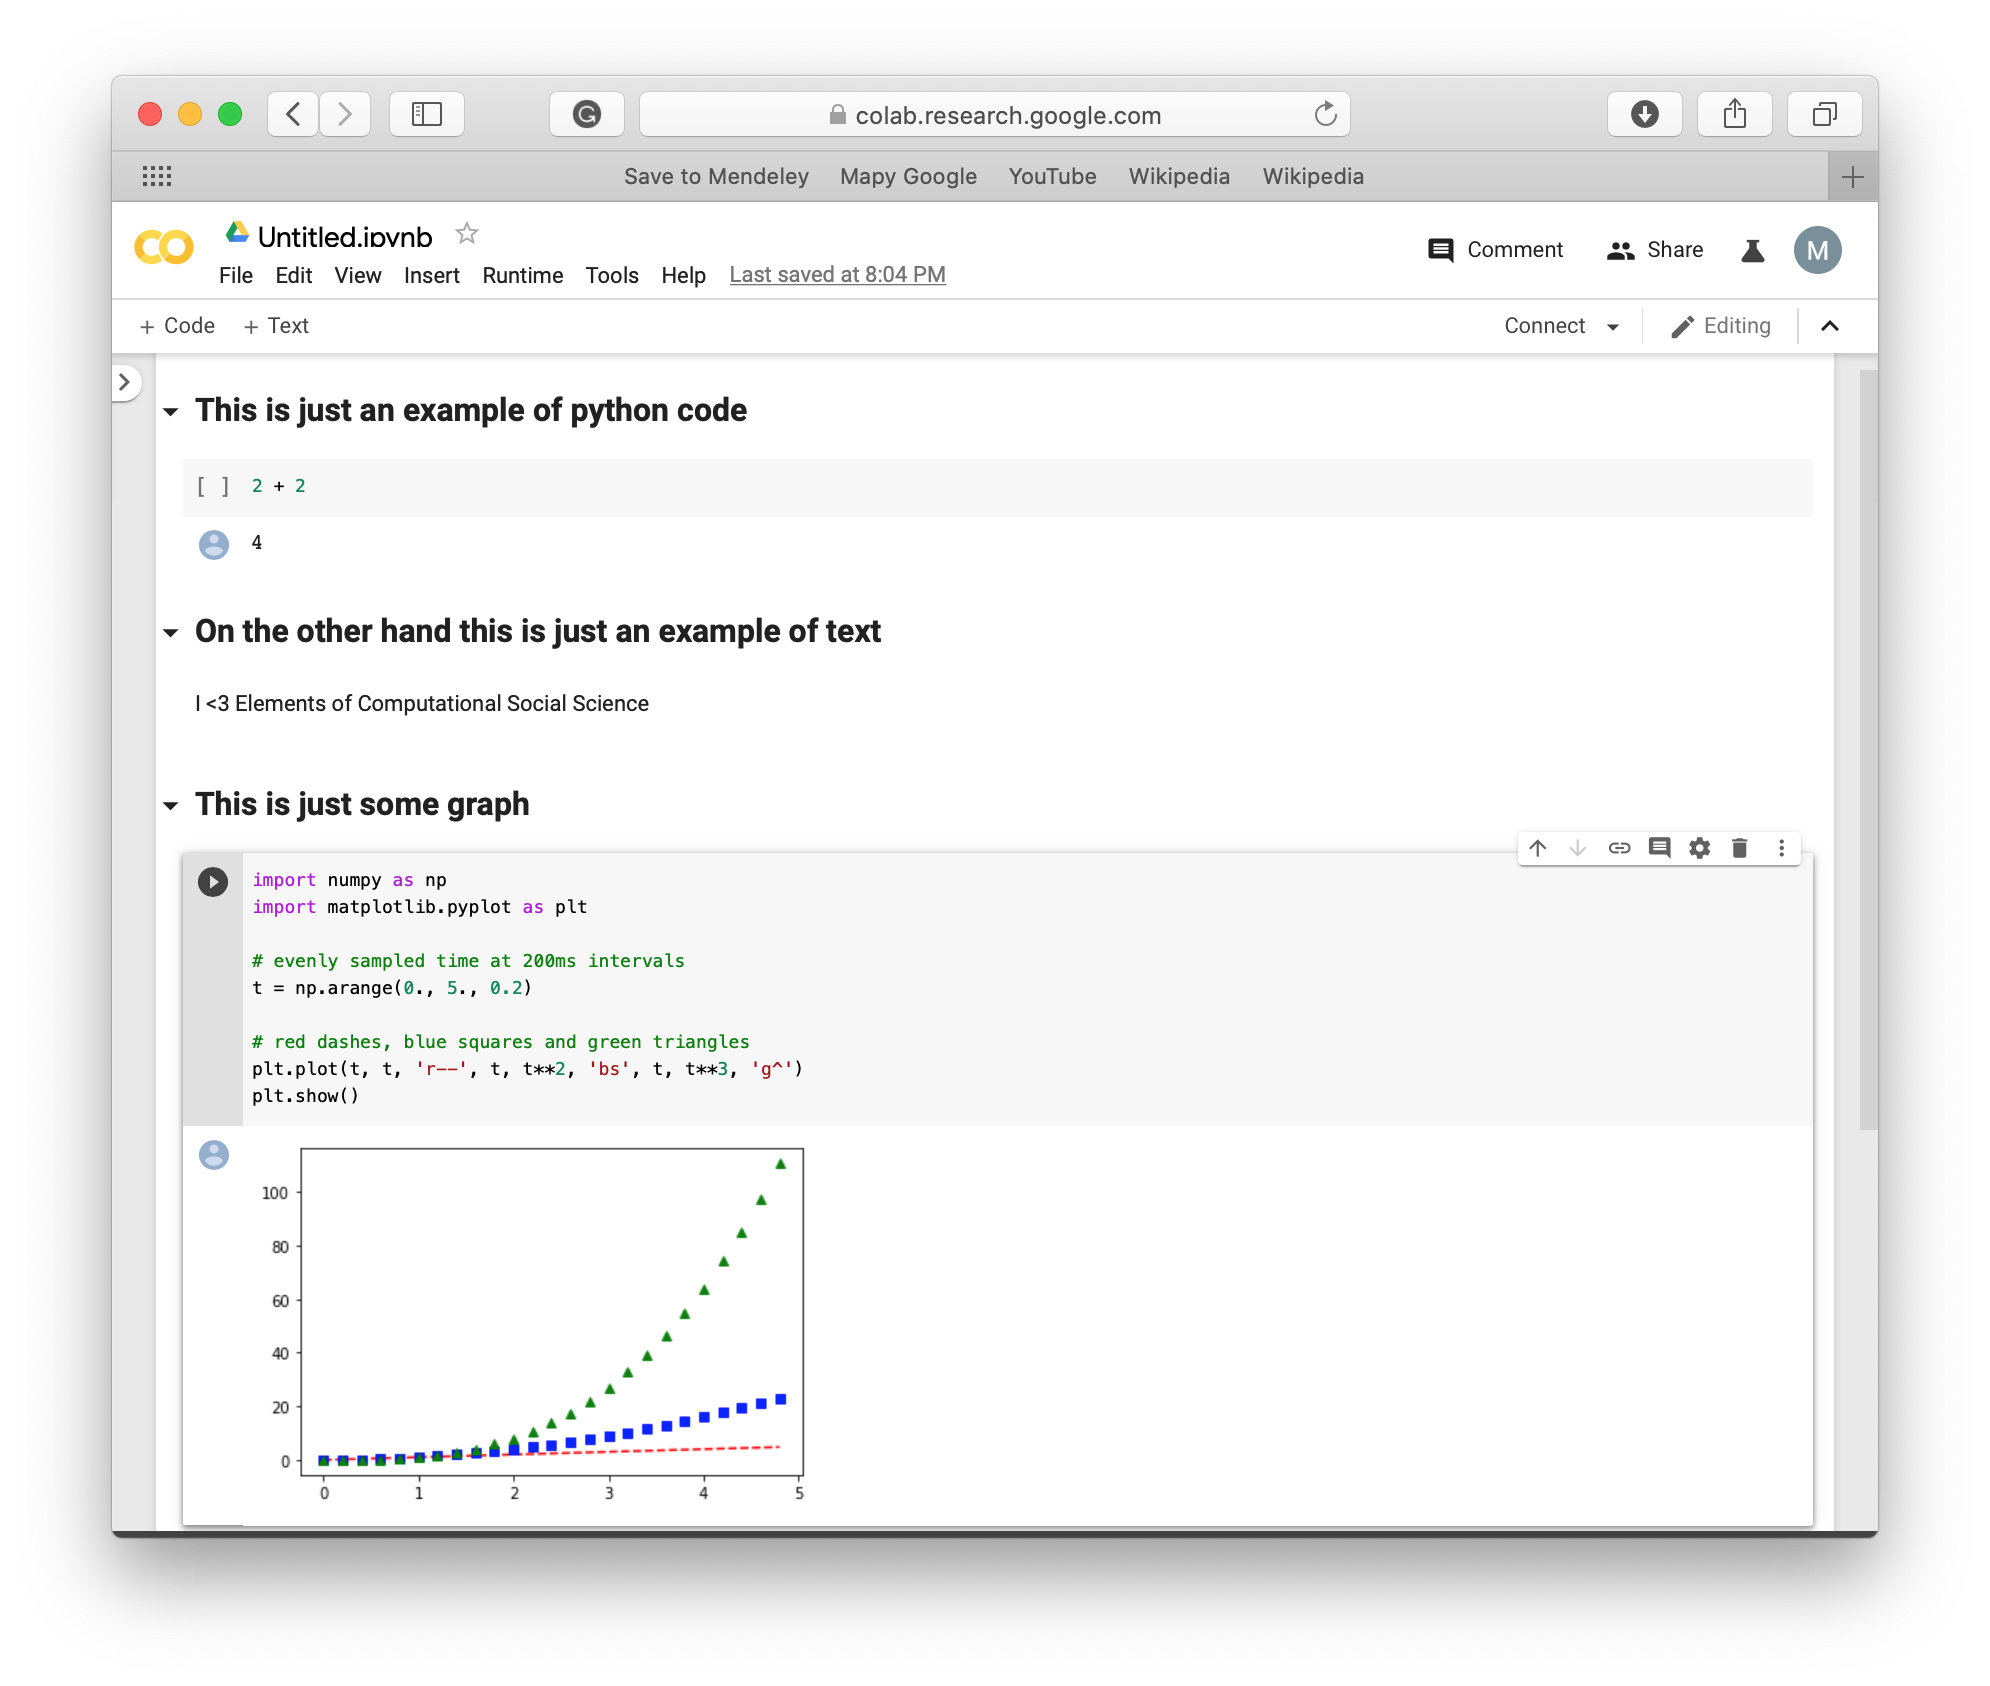
\includegraphics[width = \framewidth]{png/colaboratory.png}
    }
    \only<+>{
        \frametitle{How to open Jupyter Notebook in Colaboratory?}
        If you have a google account and all of you have you just need to follow these four easy steps to open a notebook we prepared for today:
        \begin{enumerate}
            \item Visit \textcolor{blue}{\href{https://colab.research.google.com/notebooks/welcome.ipynb}{www.colab.research.google.com}}
            \item Press File and choose Open notebook\dots
            \item Choose GitHub and type \mintinline{bash}{sztal}
            \item Click on \mintinline{bash}{notebooks/jupyter/C3.ipynb}
        \end{enumerate}
    }
    \only<+>{
        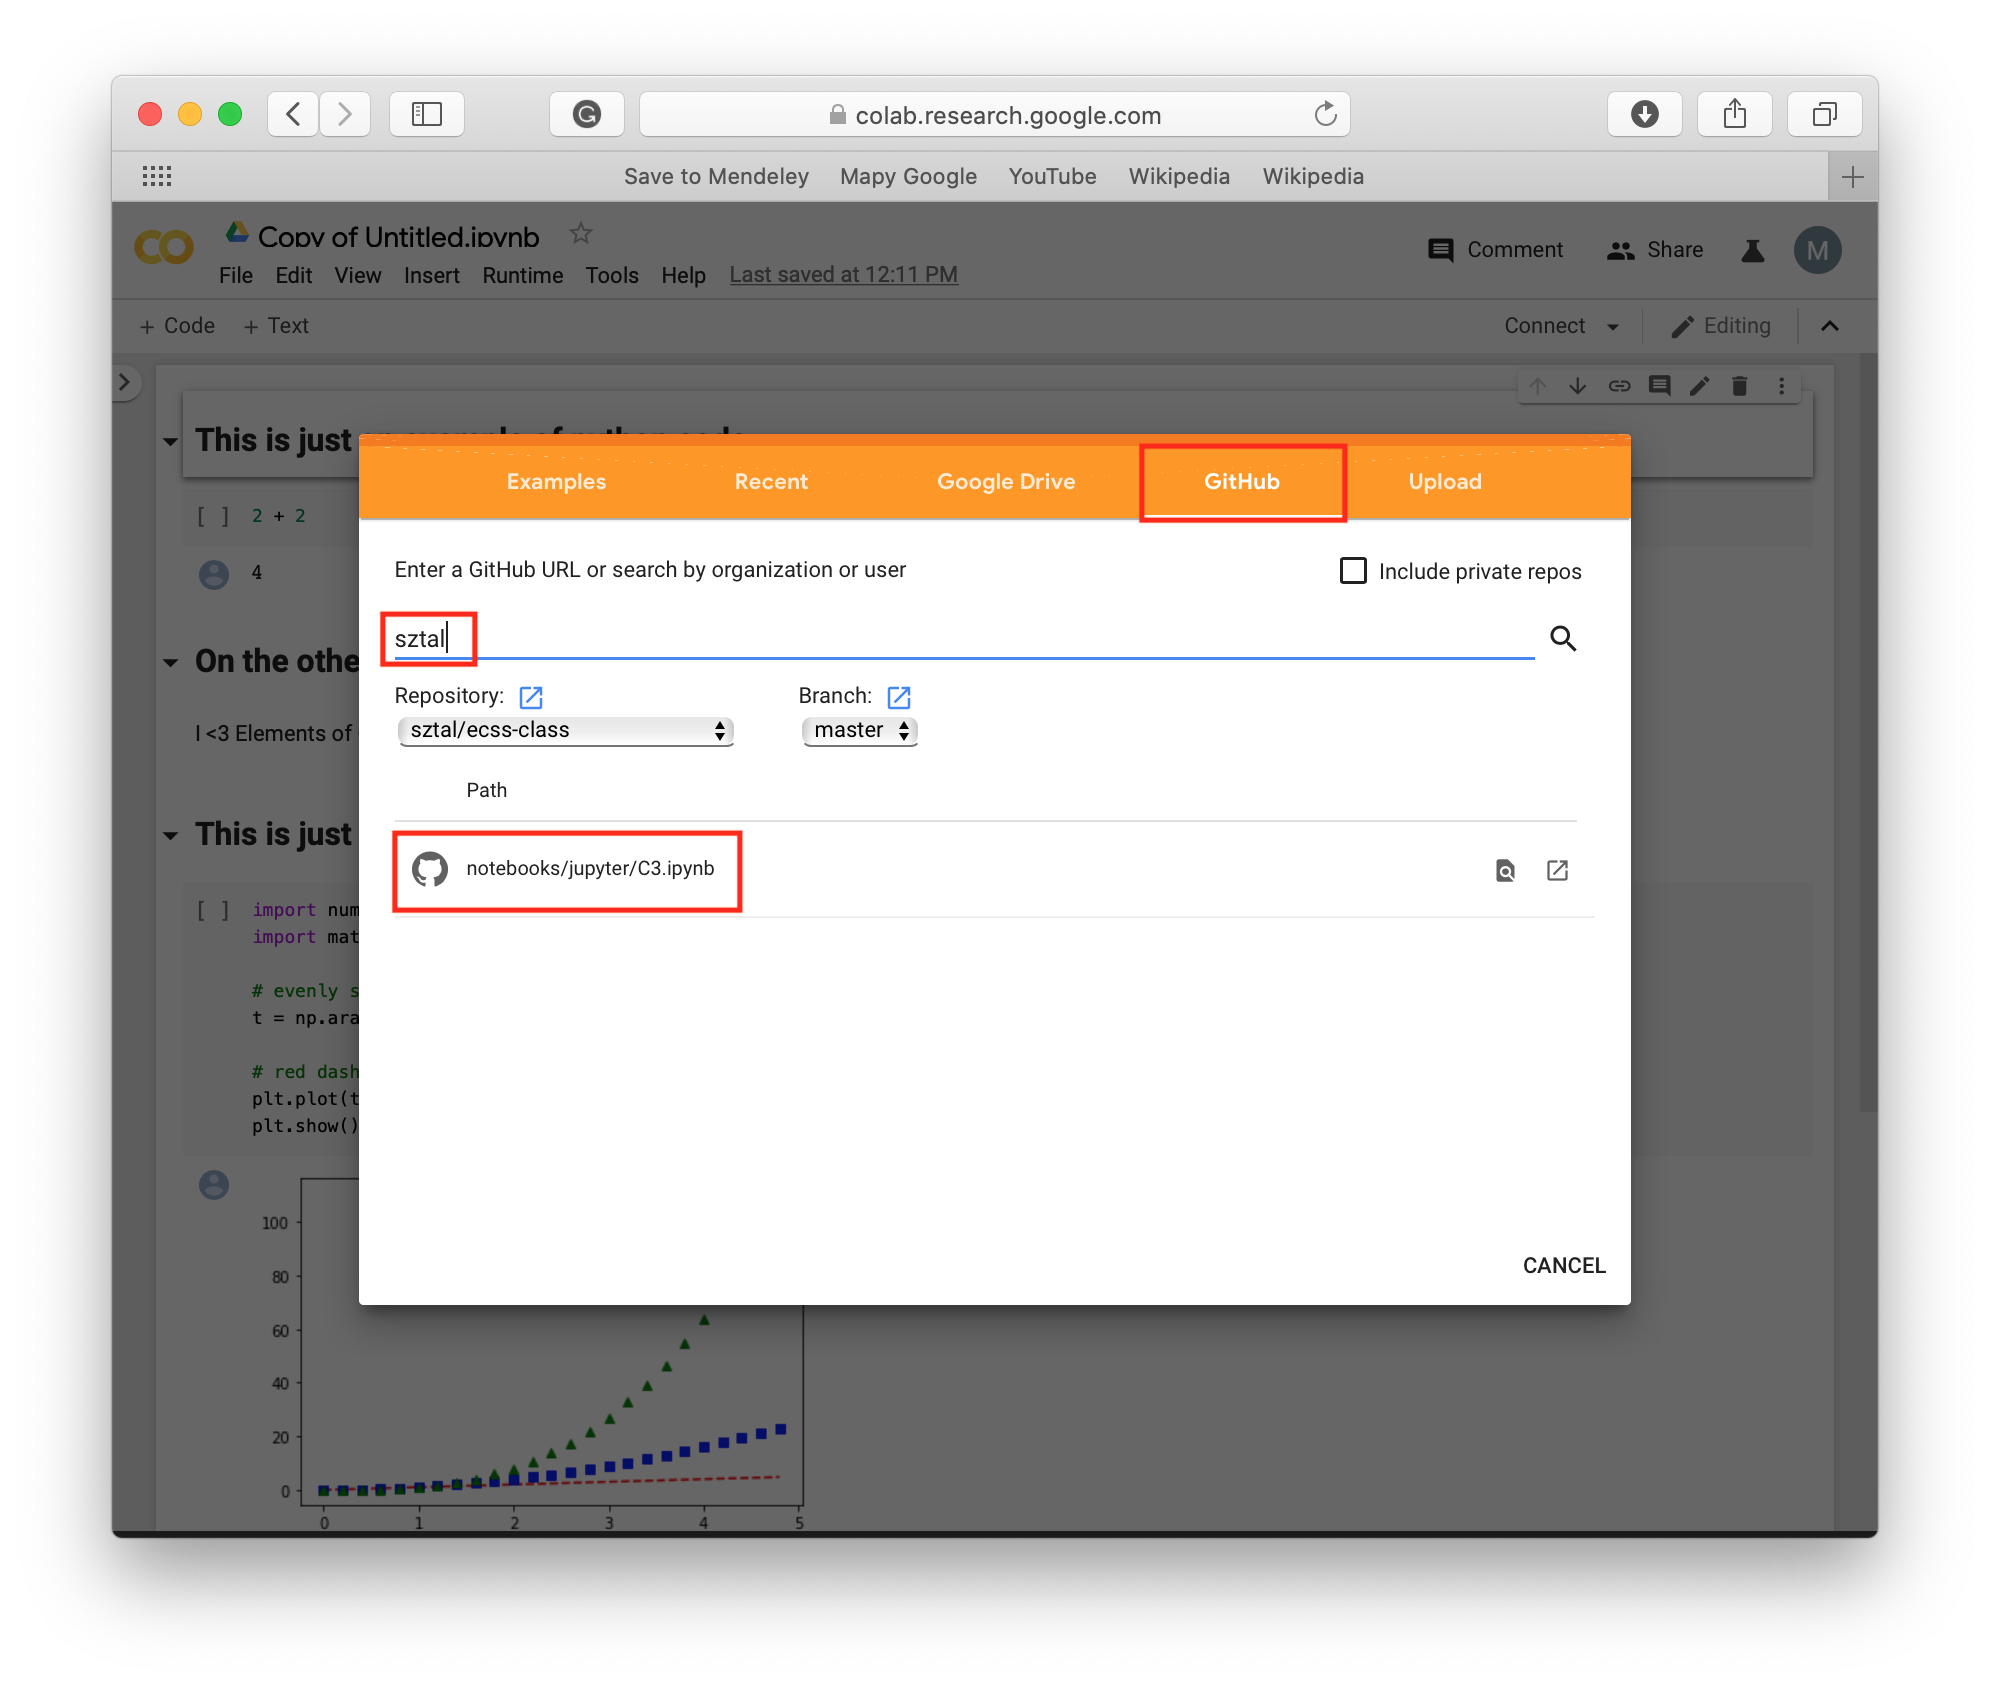
\includegraphics[width = \framewidth]{png/colab_notebook.png}
    }
\end{frame}

\subsection[Anaconda]{Anaconda}
\begin{frame}[fragile]
    \only<1>{
        
\includegraphics[width = \framewidth]{png/anaconda.png}
    }
    \only<2>{
        \frametitle{What is Anaconda?}
        \begin{definition}
            \emph{Anaconda} is a free and open-source distribution of Python and R programming languages for scientific computing that aims to simplify package management and deployment. It comes with more than 1500 packages installed and conda package and virtual environment manager.
        \end{definition}
    }
    \only<3>{
        \frametitle{What is Conda?}
        \begin{definition}
            \emph{Conda} is an open-source, cross-platform, package manager and environment management system. In other words, it allows to easily download new packages and to create project-specific environments.
        \end{definition}
    }
    \only<4,6>{
        \frametitle{Before installing Anaconda on Mac}
        Unfortunately, installing Anaconda on the new macOS became a bit tricky especially if you already had Anaconda installed when you updated to macOS Catalina. Anyway, before you go any further (no matter what macOS you have) follow these three steps:
        \begin{enumerate}
            \item<4,6> Press \mintinline{bash}{cmd} and \mintinline{bash}{space} at the same time
            \item<4,6> Type Terminal and press \texttt{return (enter)}
            \item<6> Type \mintinline{bash}{xcode-select --install} and press RETURN (ENTER)
        \end{enumerate}
    }
    \only<5>{
        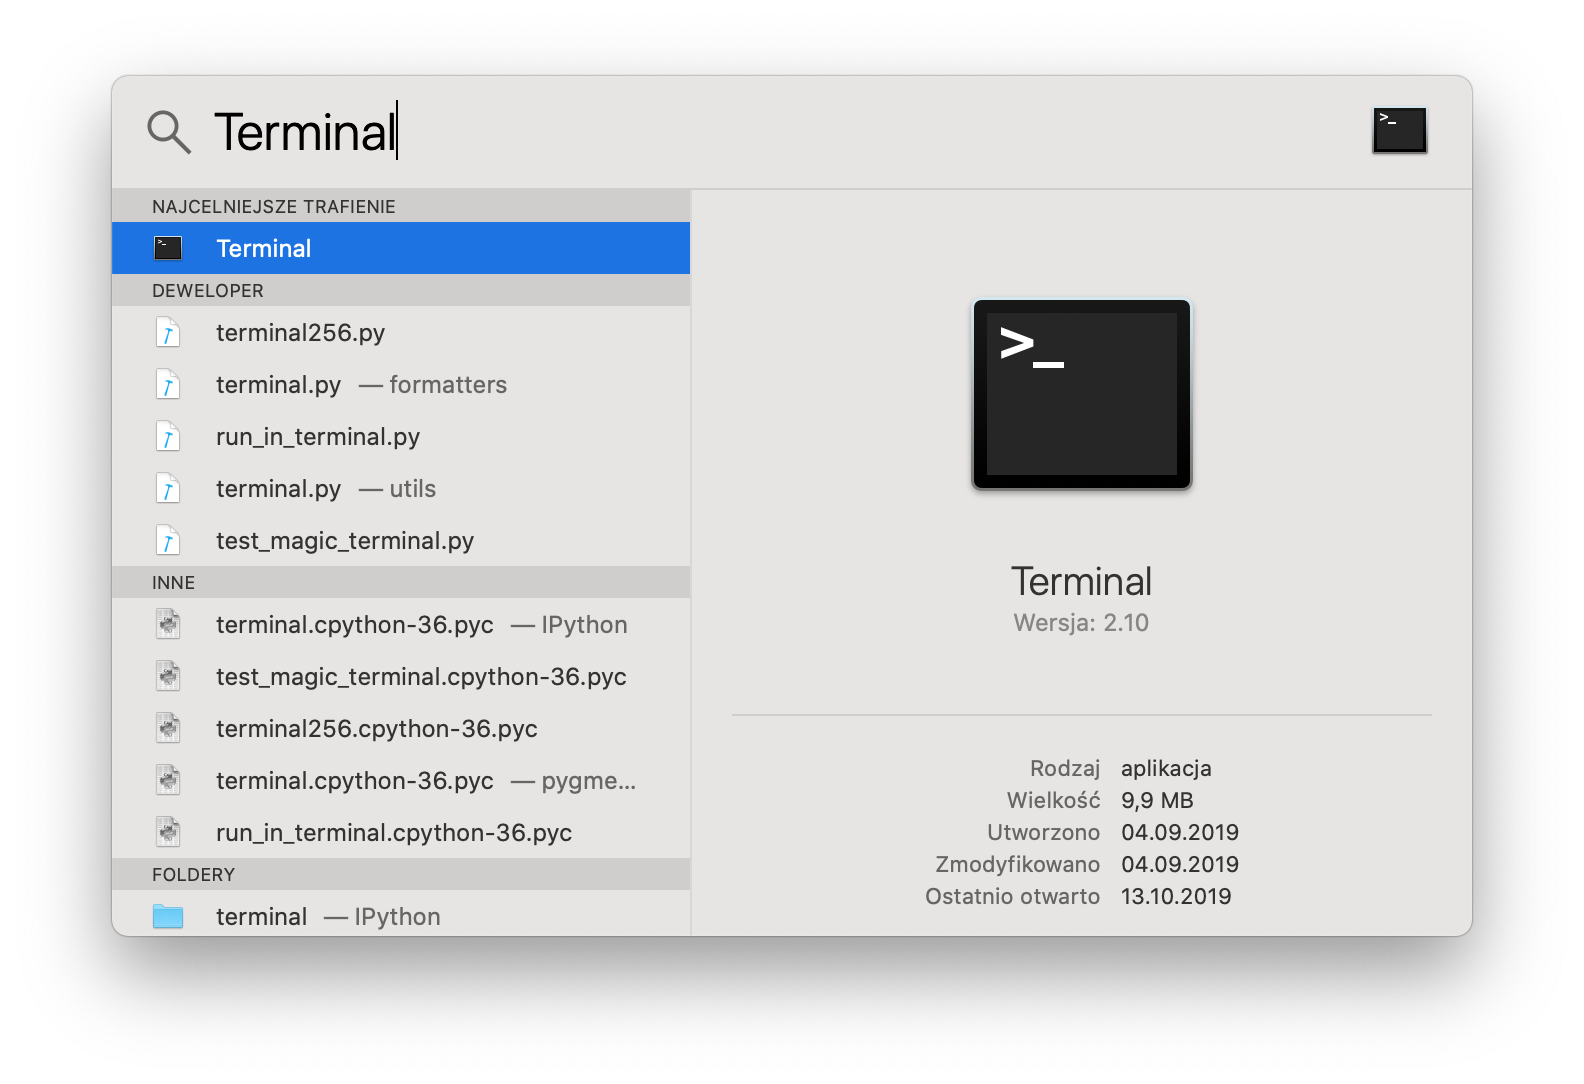
\includegraphics[width = \framewidth]{png/spotlight.png}
    }
    \only<7>{
        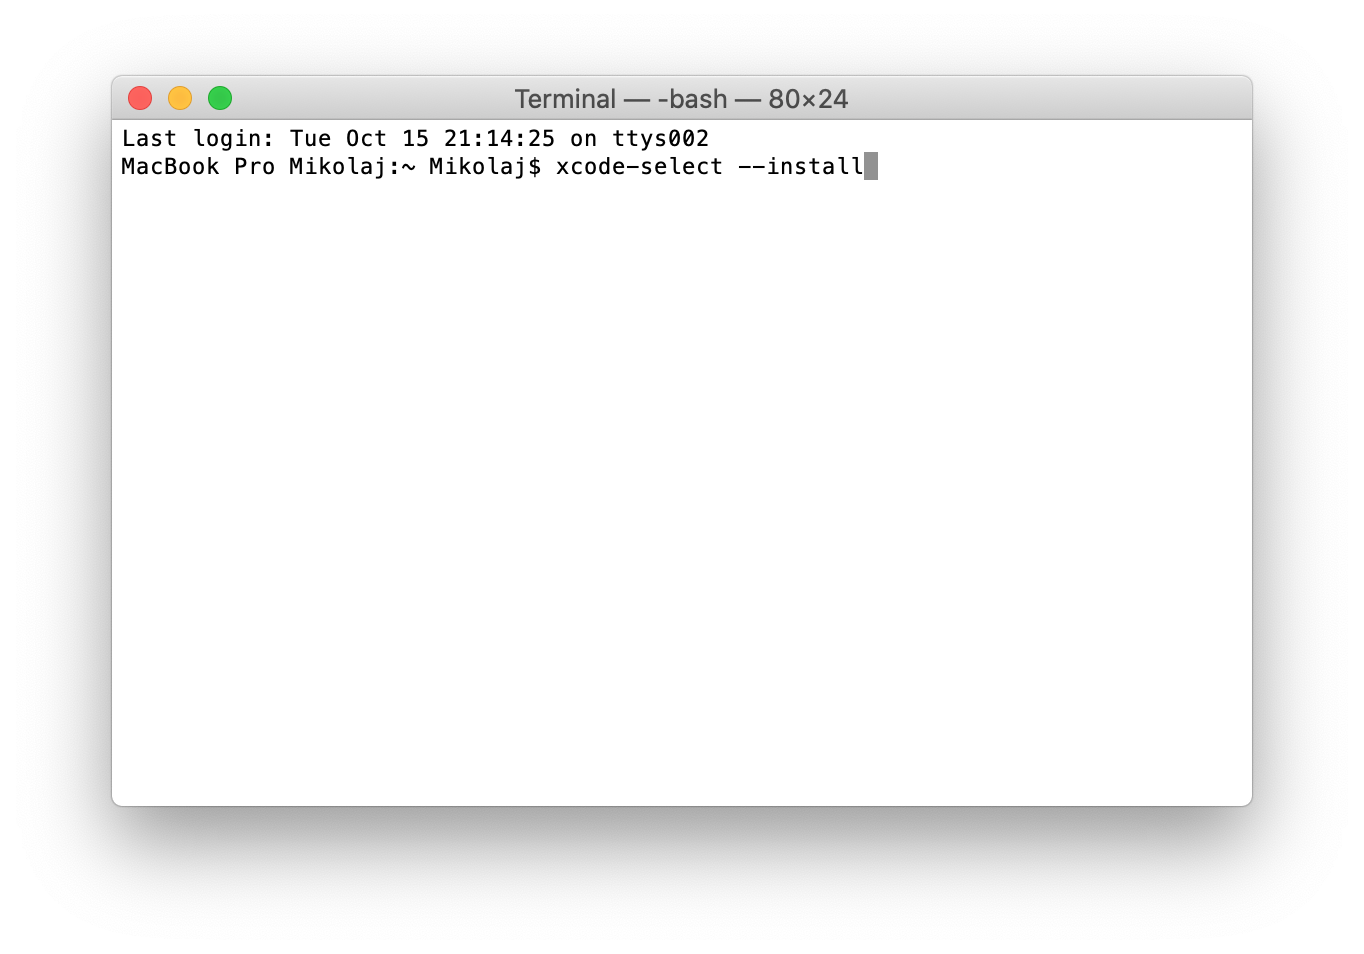
\includegraphics[width = \framewidth]{png/terminal.png}
    }
    \only<8,10,12>{
        \frametitle{How to install Anaconda on Mac?}
        Now, to install Anaconda just follow these five steps:
        \begin{enumerate}
            \item<8,10,12> Visit \textcolor{blue}{\href{https://www.anaconda.com}{www.anaconda.com}}
            \item<8,10,12> Click download and scroll down to choose version
            \item<8,10,12> Download Python 3.7 version 64-Bit Command Line Installer
            \item<10,12> Type \mintinline{bash}{bash ~/Downloads/Anaconda3-2019*.sh} in Terminal and press \texttt{return (enter)}
            \item<12> Type \mintinline{bash}{jupyter notebook} in Terminal and press \texttt{return (enter)} to open the Jupyter Notebook App
        \end{enumerate}
    }
    \only<9>{
        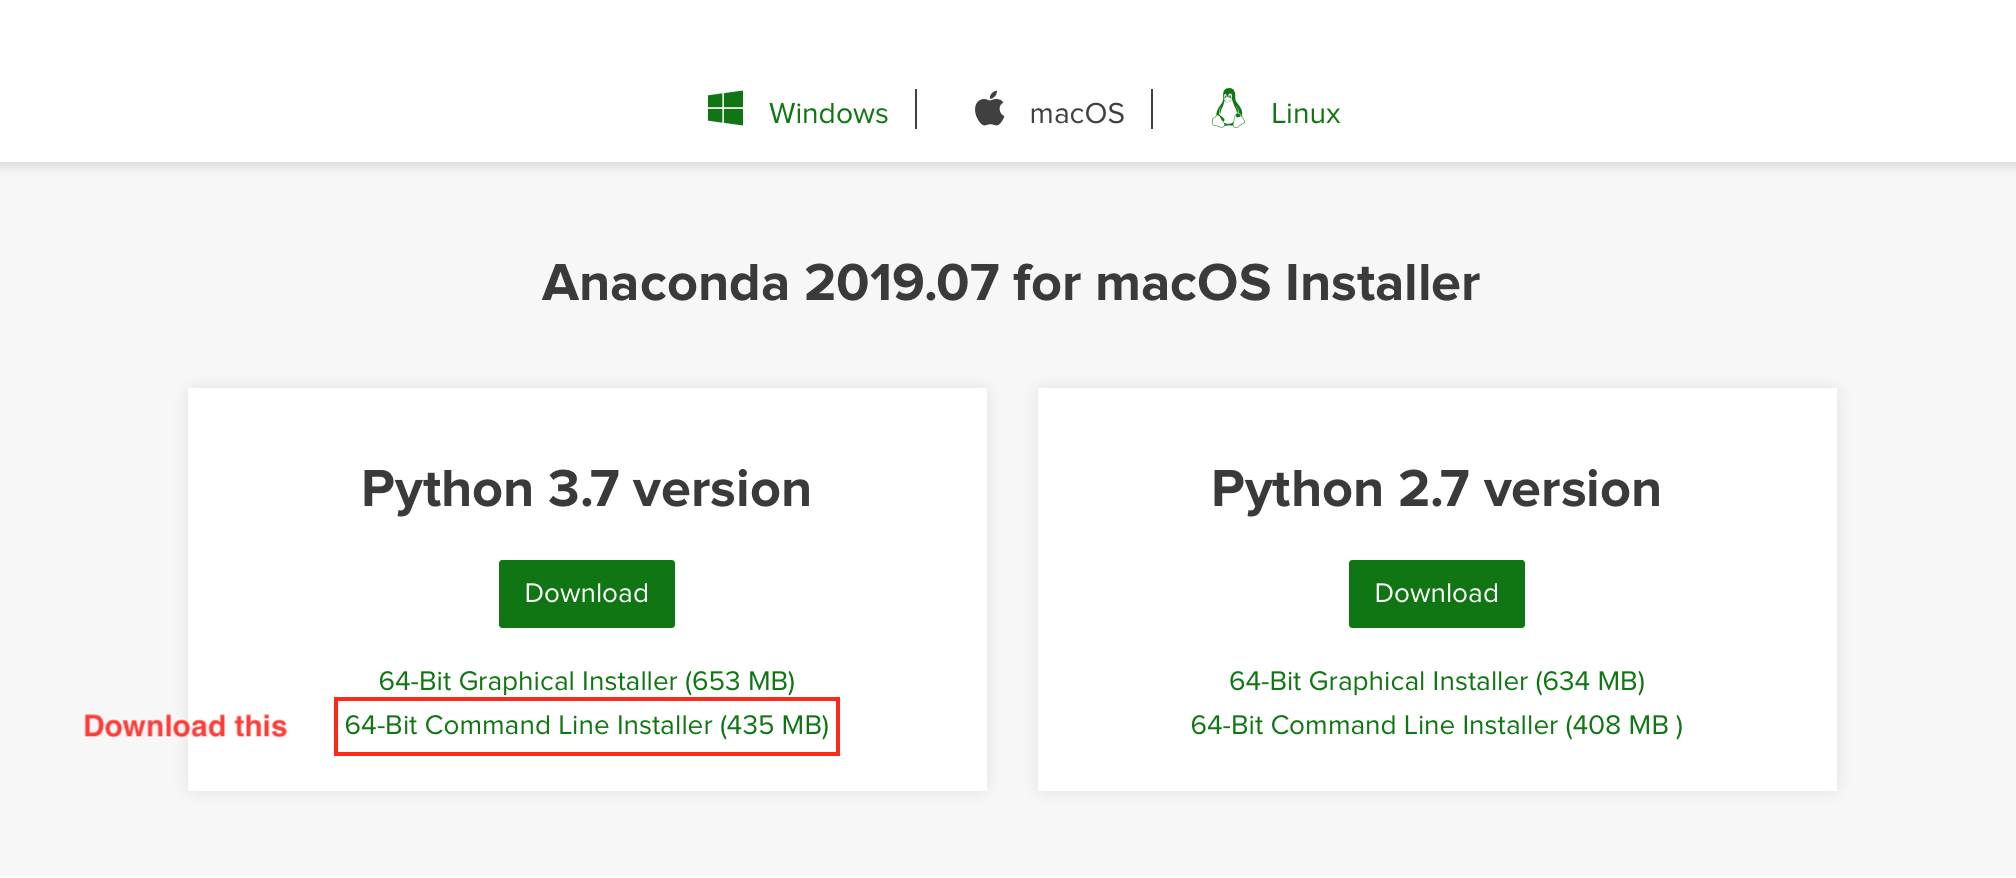
\includegraphics[width = \framewidth]{png/anaconda_installer_mac.png}
    }
    \only<11>{
        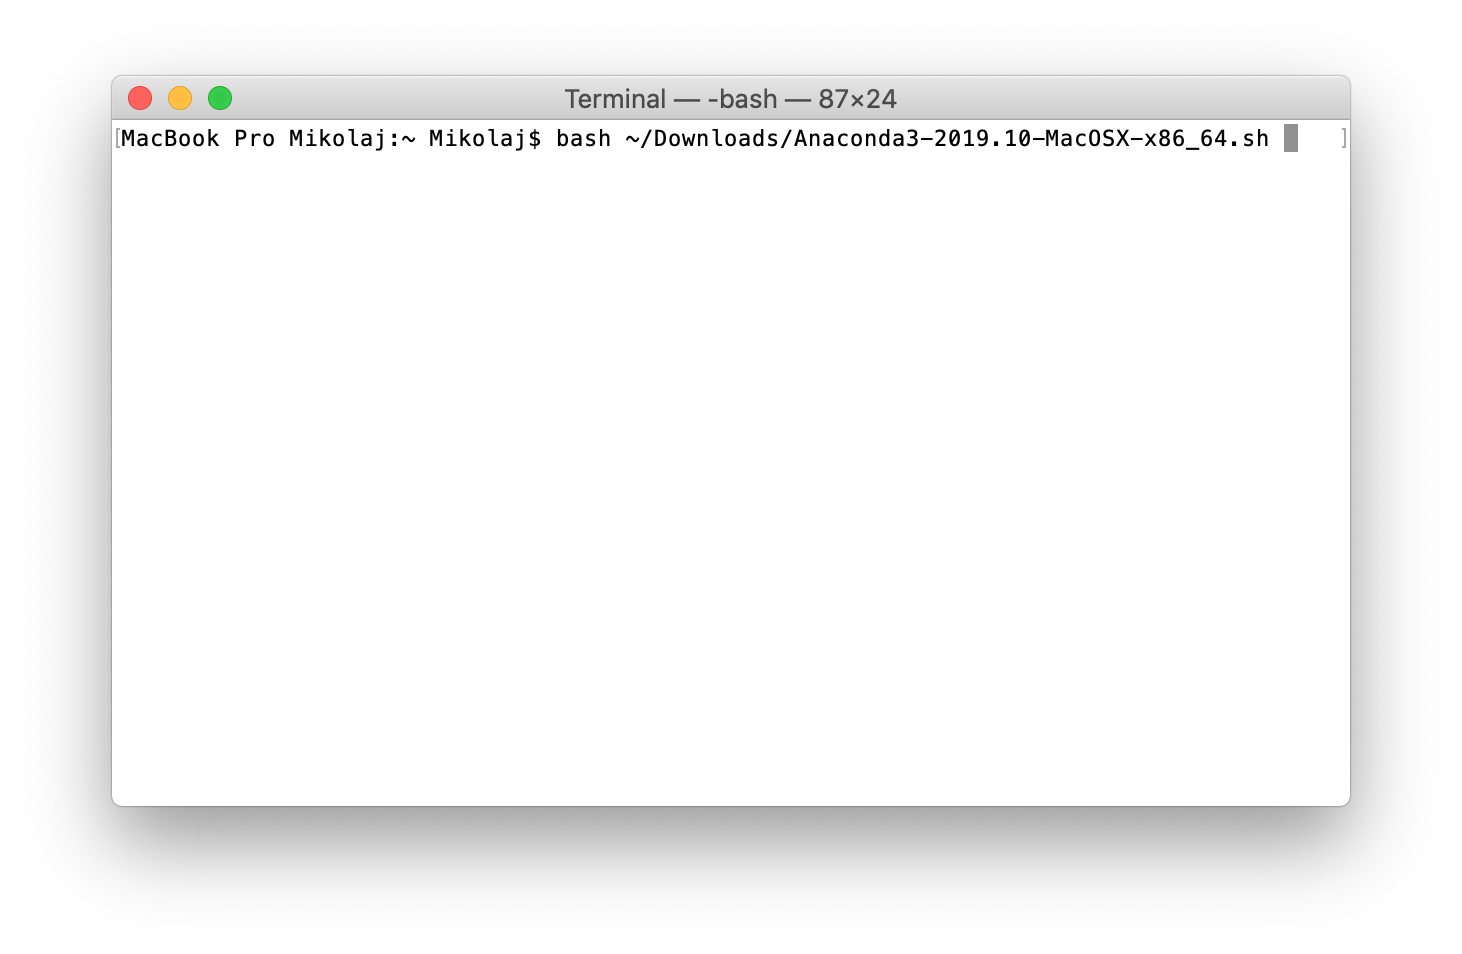
\includegraphics[width = \framewidth]{png/terminal_install.png}
    }
    \only<13>{
        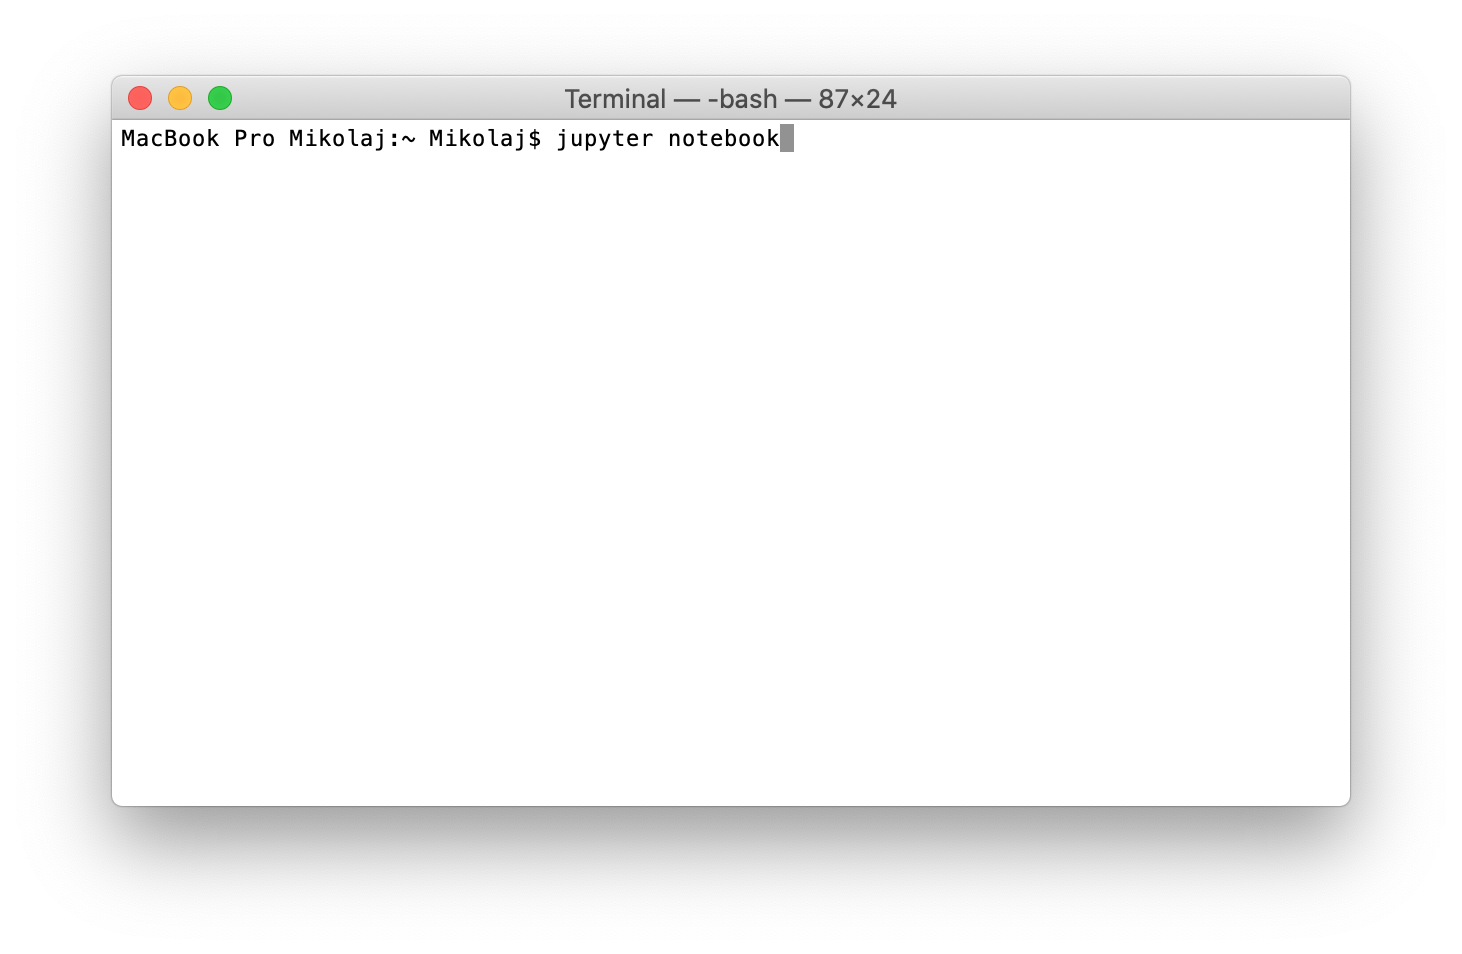
\includegraphics[width = \framewidth]{png/terminal_notebook.png}
    }
    \only<14,16>{
        \frametitle{How to install Anaconda on Windows}
        Installing Anaconda on Windows should be relatively easy:
        \begin{enumerate}
            \item<14,16> Visit \textcolor{blue}{\href{https://www.anaconda.com}{www.anaconda.com}}
            \item<14,16> Click download and scroll down to choose version
            \item<14,16> Download Python 3.7 64-Bit Graphical Installer
            \item<14,16> Double click on \texttt{Anaconda3-2019.10-Windows-x86\_64.exe} and follow the default installation
            \item<16> Type \mintinline{bash}{jupyter notebook} in Anaconda Prompt and press \texttt{enter} to open Jupyter Notebook
        \end{enumerate}
    }
    \only<15>{
        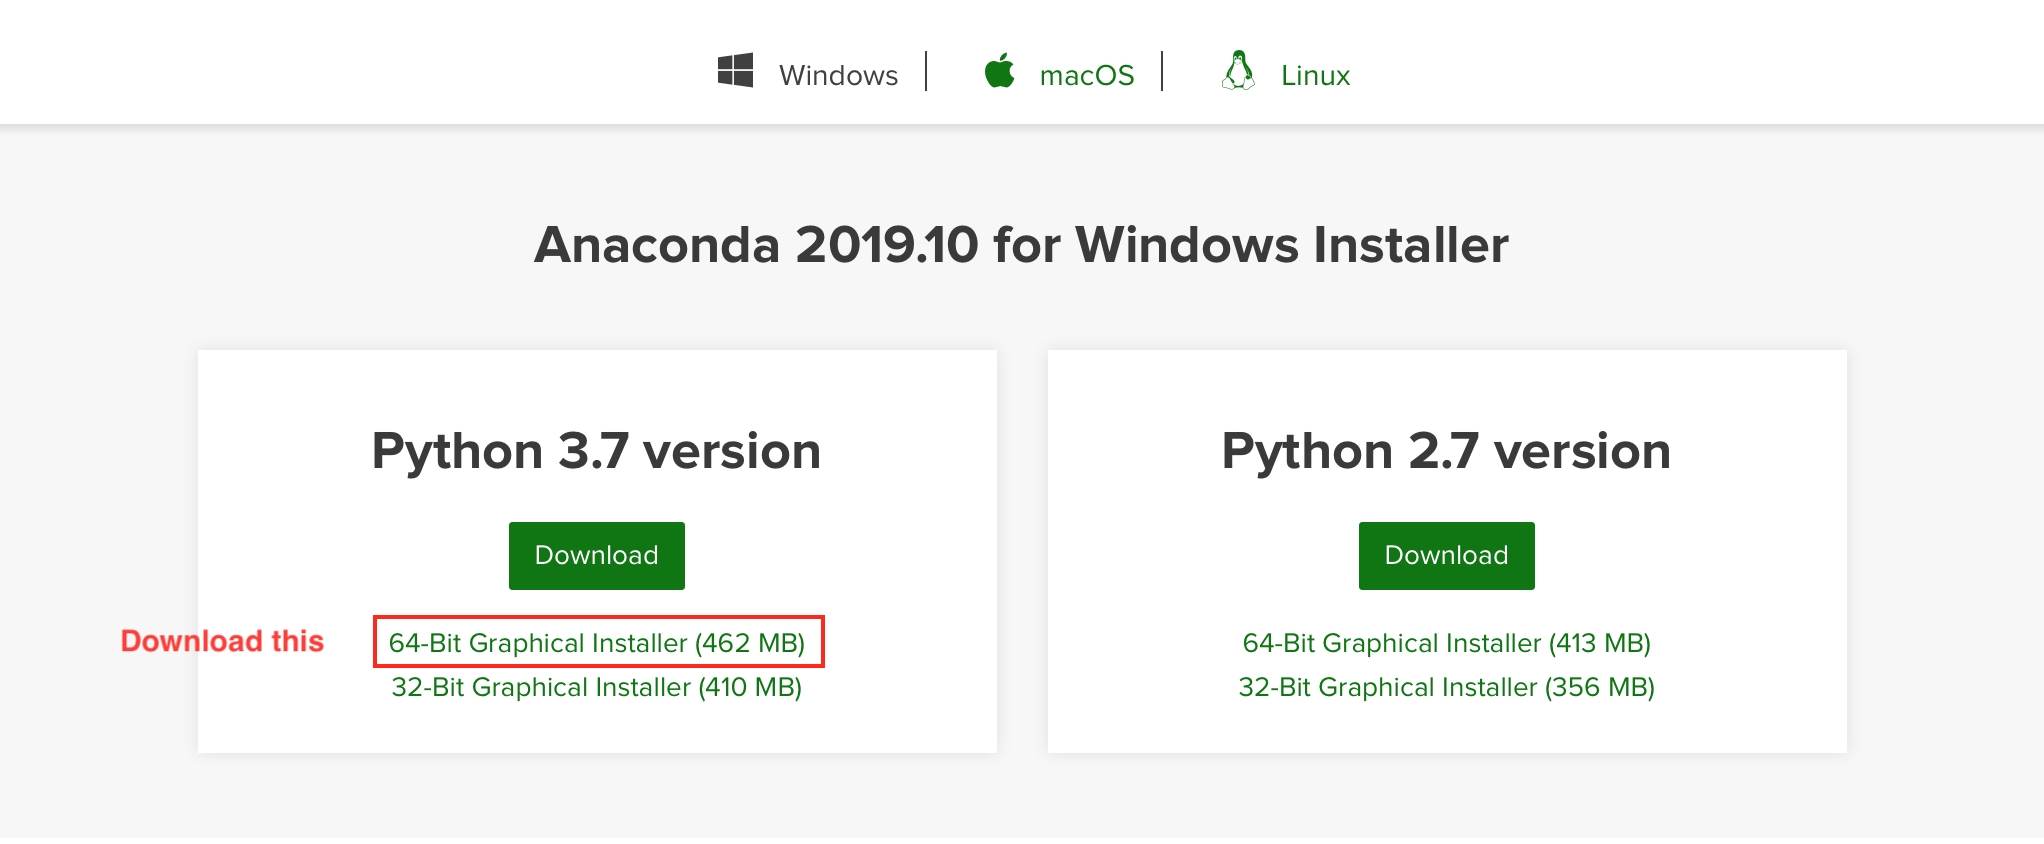
\includegraphics[width = \framewidth]{png/anaconda_installer_win.png}
    }

\end{frame}


